\section{Techniques to Improve Precision on \mH Measurement}
\label{sec:techniques}

% %=== Hualin's thesis ===%
% % \subsubsection{Computation of Per-Event Mass Uncertainties}
% % \subsubsection{Correction of Lepton Momentum Uncertainties}
% % \subsubsection{Model and Procedure to Derive Corrections}
% % \subsubsection{Validation of Corrections}
% %=== AN-19-248 ===%
% % \subsubsection{motivation}
% % \subsubsection{model and procedure to derive Corrections}
% % \subsubsection{validation of corrections (MC, data)}

% \subsection{Matrix Element-Based Kinematic Discriminant}

% \begin{table}[ht]
%     \begin{center}
%     \begin{tabular}{|c|cccc|c|}
%     \hline			
%     Expected uncertainty	&	4$\mu$	&	4e	&	2e2$\mu$	&2$\mu$2e	& Inclusive	\\
%     \hline			
%         1D	(No bkg) &	153	&	466	&	315	&	300	&	121	\\
%     \hline
%     \end{tabular}
%     \end{center}
%     \caption{
%         %=== Below is the description from AN-19-248. ==%
%         % Expected Higgs boson mass uncertainty measured with 1D model 
%         % for different final states. All mass values are given in \MeV.
%         % Statistical-only results are considered at this stage of the analysis.
%         }
%     \label{table:model_result_fs_1D}
%     \end{table}

Several analysis techniques---some old and some new with respect to the 2016 measurement of \mH by CMS TODO:Ref HIG-16-041---help to improve the precision on \mH.
Each technique is individually described in the sections that follow.

% TODO: make mfourl bold here but not in TOC.
% TODO: check out sec-075-newEBE.tex
% \subsection{Per-Event Relative Mass Error Categorization}
\subsection{Improving Event-by-Event \mfourl Uncertainty}
\label{sec:ebe}
% TODO:REWORD
For each event, the uncertainty on the \mfourl value (\mfourlerr) is used directly in the \Zone constraint (Sec.~\ref{sec:Z1constraint}).
By improving the precision on the \mfourlerr 
Per-event four-lepton uncertainties are used for (a) performing the \Zone constraint and (b) in the measurement of \mH so that better-measured events are given higher weights in the likelihood fit.
Individual lepton uncertainty on momentum measurement can be predicted on a per-lepton 
basis. In the case of muons, the full error matrix is obtained using muon track fit; for the electrons,
instead, the momentum error is estimated from the combination of the ECAL and tracker measurement, 
neglecting the uncertainty on the track direction from the GSF fit. \\
The uncertainty on the kinematics at the per-lepton level is then propagated to the four-lepton case 
to predict the mass error on an event-by-event basis, using the following approach.\\
Each $\delta m_{i}$, corresponding to individual lepton momentum variation, is calculated separately 
and then the measured resolution on the invariant mass of the four leptons is taken as the quadrature sum 
of the four individual $\delta m_{i}$:
\[
m_{0} = F(p_{T1}, \phi_{1},\eta_{1}; p_{T2}, \phi_{2},\eta_{2}; p_{T3}, \phi_{3}, \eta_{3}; p_{T4}, \phi_{4},\eta_{4})
\]
\[\delta m_{i} = F(...; p_{Ti} + \delta p_{Ti}, \phi_{i}, \eta_{i}; ...) - m_{0} \quad
\]
\[
\delta m = \sqrt{\delta m_{1}^2 + \delta m_{2}^2 + \delta m_{3}^2 + \delta m_{4}^2}
\]

%=== Can't get the below to be centered...
% \begin{align*}
%         m_0 = F(
%         p_{T1}, \phi_1, \eta_1;
%         p_{T2}, \phi_2, \eta_2;
%         p_{T3}, \phi_3, \eta_3;
%         p_{T4}, \phi_4, \eta_4
%         )
%         \\
%         \delta m_i = F(...; p_{Ti} + \delta p_{Ti}, \phi_i, \eta_i; ...) - m_0
%         \\
%         \delta m = \sqrt{
%         (\delta m_1)^2 + (\delta m_2)^2 + (\delta m_3)^2 + (\delta m_4)^2
%         }
% \end{align*}
% TODO: Check with Filippo if these are MC or data.
The full error matrices ($\delta p_{T}/p_{T}$, $\eta$) for muons and electrons, separately, are shown in Fig.~\ref{fig:2D_Mpas_vs_eta} for all years.
\begin{multiFigure}
    \centering

    \addFigure{0.32}{../../higgsmassmeasurement/AN-19-248/Figures/EBE/2016_vs_eta_muon_workinprogress.pdf}
    \addFigure{0.32}{../../higgsmassmeasurement/AN-19-248/Figures/EBE/2016_vs_eta_ele_ECAL_workinprogress.pdf}
    \addFigure{0.32}{../../higgsmassmeasurement/AN-19-248/Figures/EBE/2016_vs_eta_ele_tracker_workinprogress.pdf}

    \addFigure{0.32}{../../higgsmassmeasurement/AN-19-248/Figures/EBE/2017_vs_eta_muon_workinprogress.pdf}
    \addFigure{0.32}{../../higgsmassmeasurement/AN-19-248/Figures/EBE/2017_vs_eta_ele_ECAL_workinprogress.pdf}
    \addFigure{0.32}{../../higgsmassmeasurement/AN-19-248/Figures/EBE/2017_vs_eta_ele_tracker_workinprogress.pdf}

    \addFigure{0.32}{../../higgsmassmeasurement/AN-19-248/Figures/EBE/2018_vs_eta_muon_workinprogress.pdf}
    \addFigure{0.32}{../../higgsmassmeasurement/AN-19-248/Figures/EBE/2018_vs_eta_ele_ECAL_workinprogress.pdf}
    \addFigure{0.32}{../../higgsmassmeasurement/AN-19-248/Figures/EBE/2018_vs_eta_ele_tracker_workinprogress.pdf}
    \captionof{figure}
        [Scatterplots of the relative \pt error \vs $\eta$]
        {Scatterplots of the relative \pt error \vs $\eta$ in data.
        \;Left column: A, D, G) Muons.
        \;Middle column: B, E, H) ECAL-driven electrons.
        \;Right column: C, F, I) Tracker-driven electrons.
        \;Top row: A, B, C) 2016.
        \;Middle row: D, E, F) 2017.
        \;Bottom row: G, H, I) 2018.
        }
    \label{fig:2D_Mpas_vs_eta}
\end{multiFigure}
% \begin{figure}[!htbp]
% 	\begin{center}
% %		\subfloat[][2016]
% %		   {		
%                     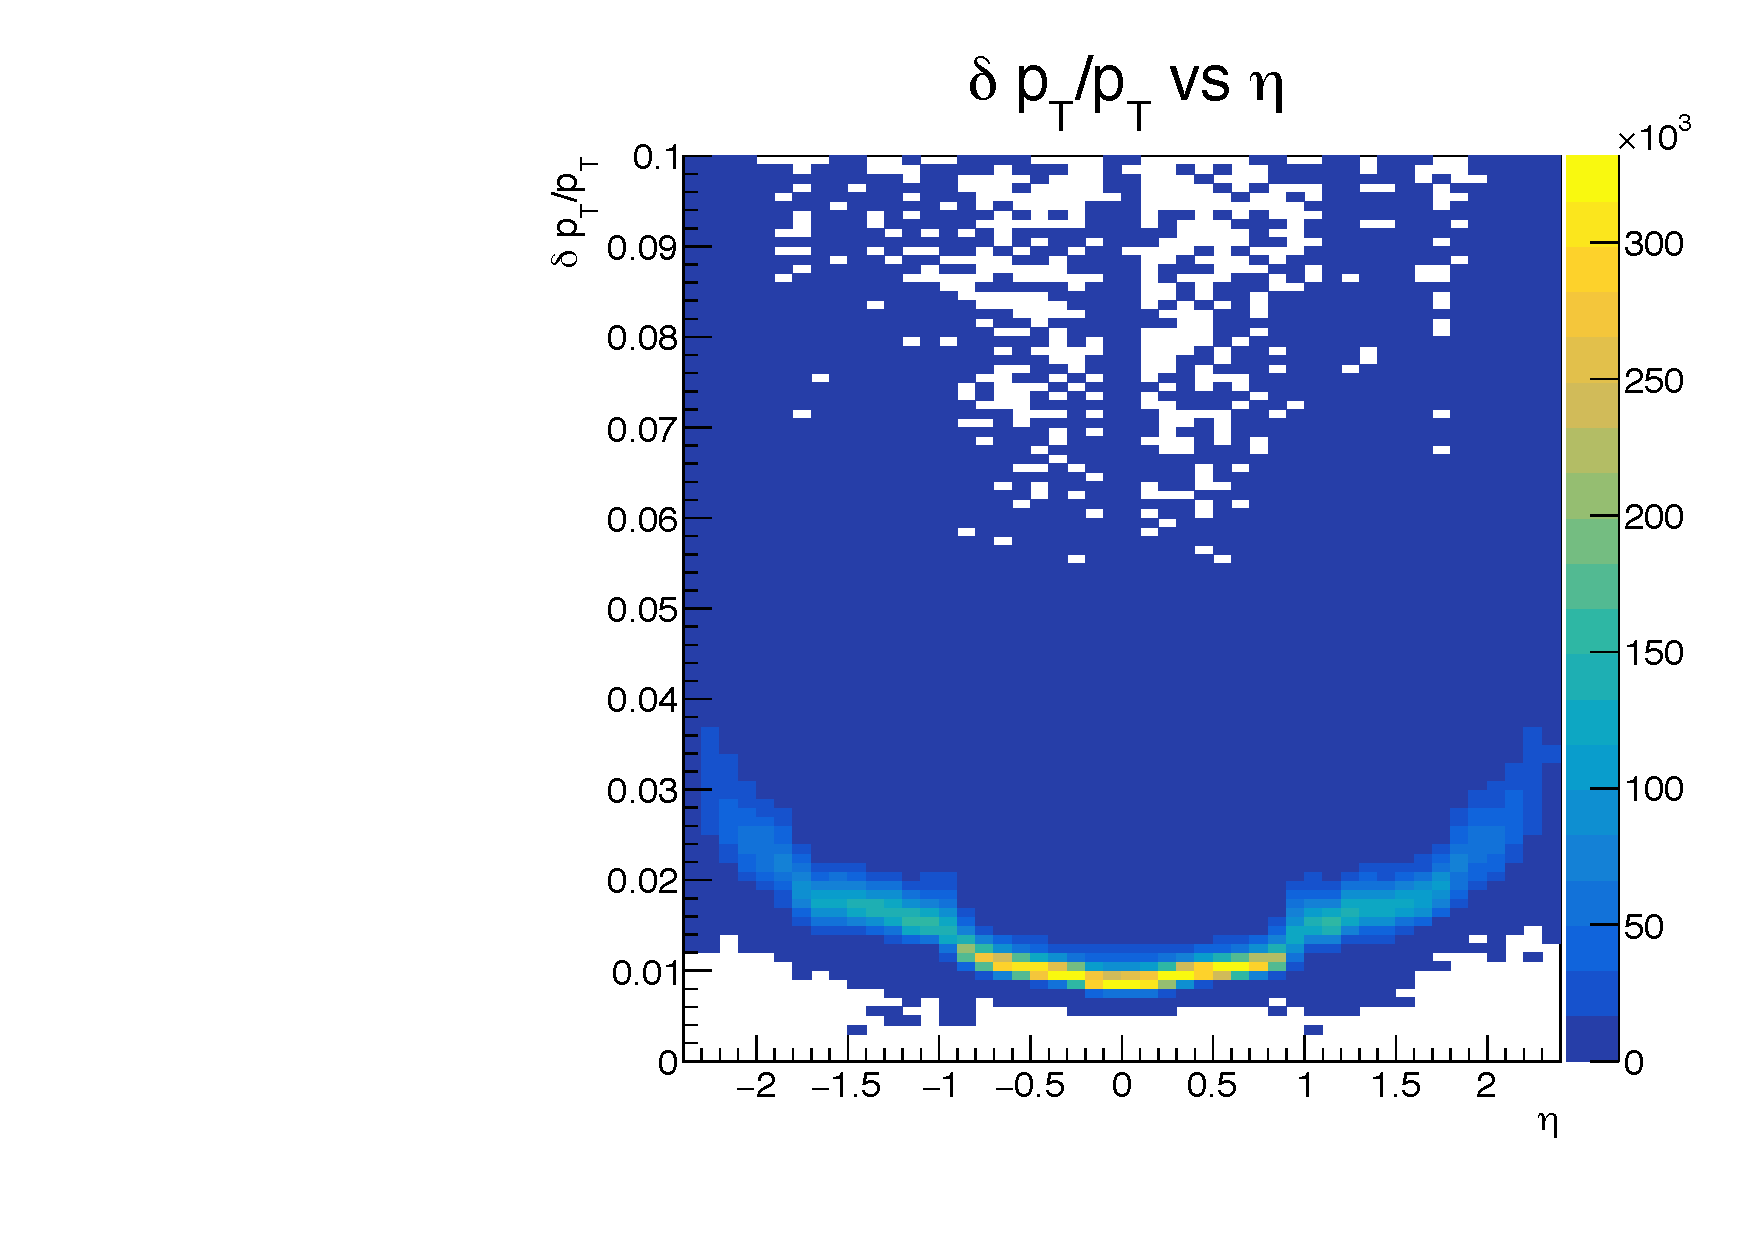
\includegraphics[width=0.32\textwidth]{Figures/EBE/2016_vs_eta_muon.pdf}
% 					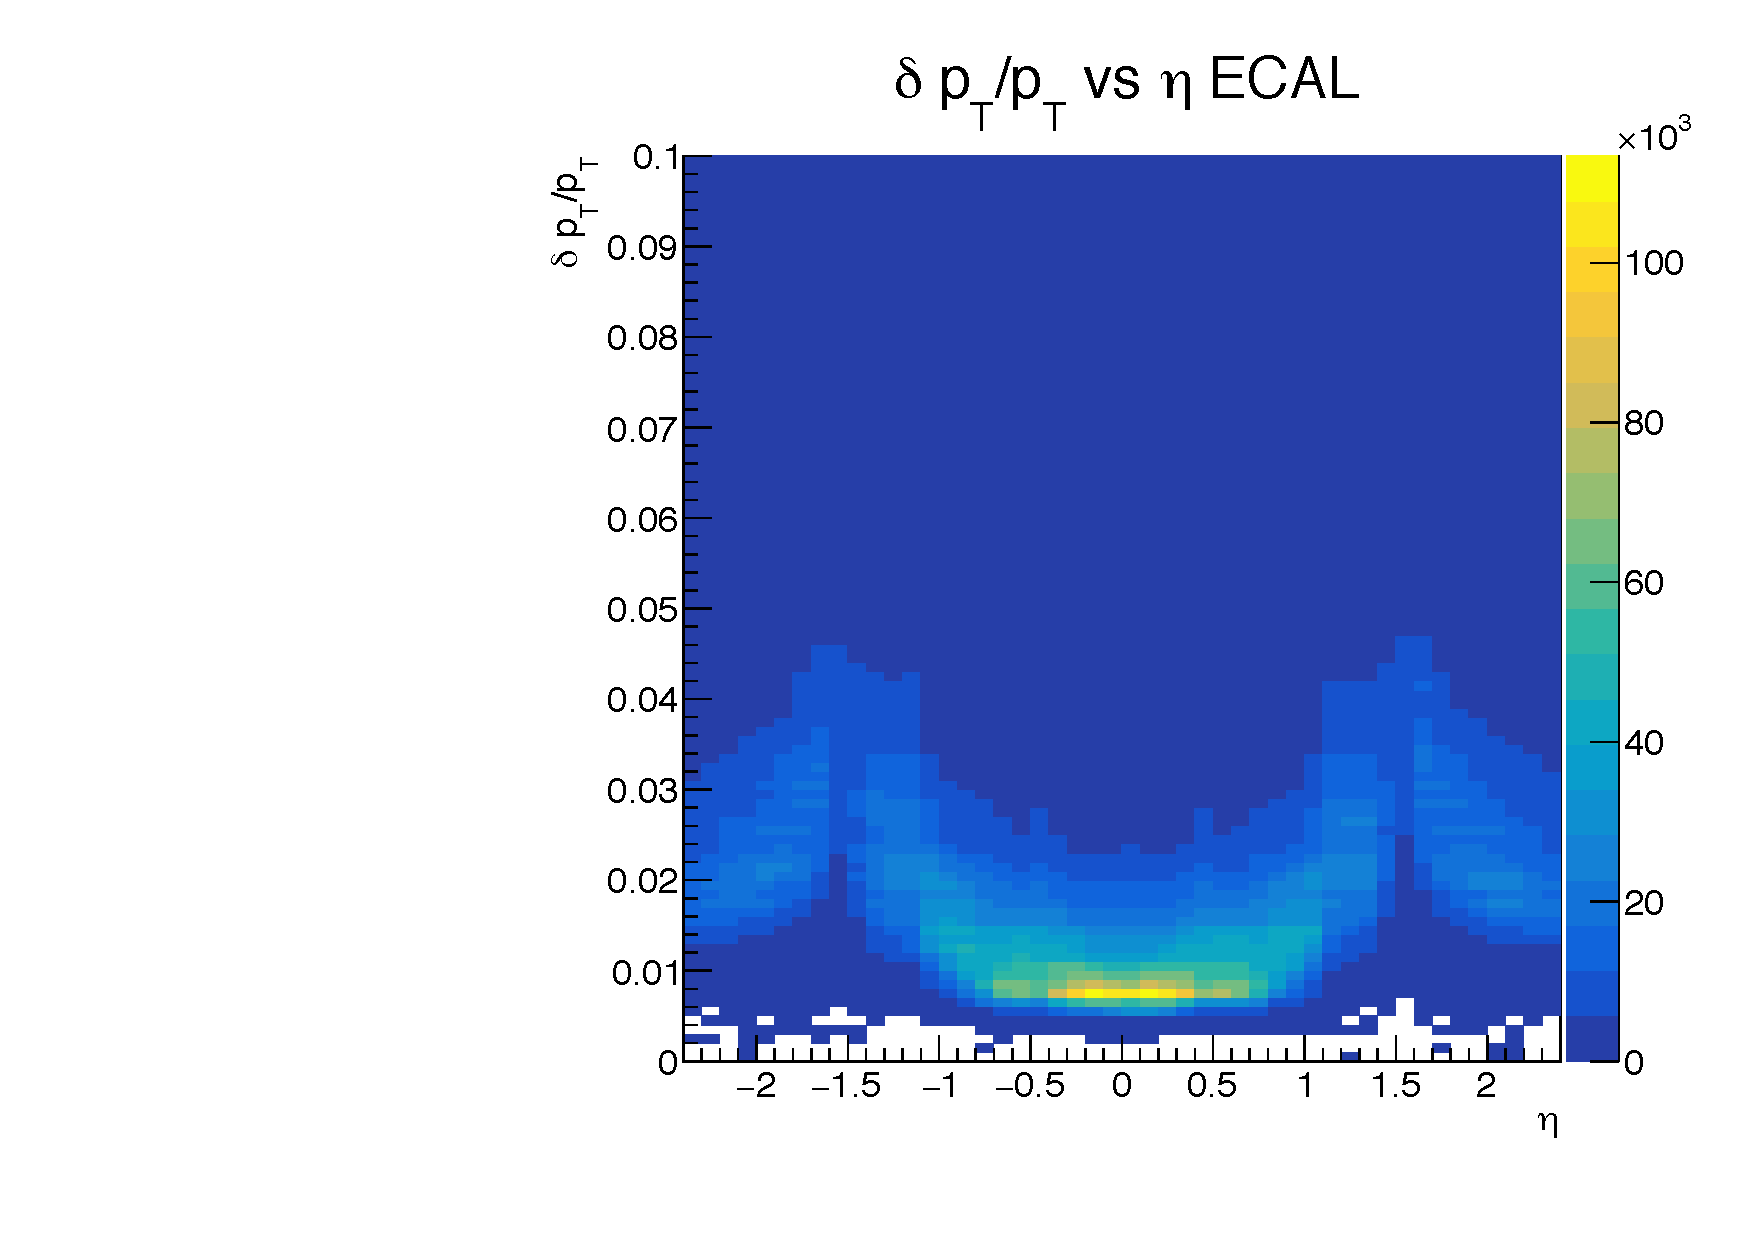
\includegraphics[width=0.32\textwidth]{Figures/EBE/2016_vs_eta_ele_ECAL.pdf} 
% 					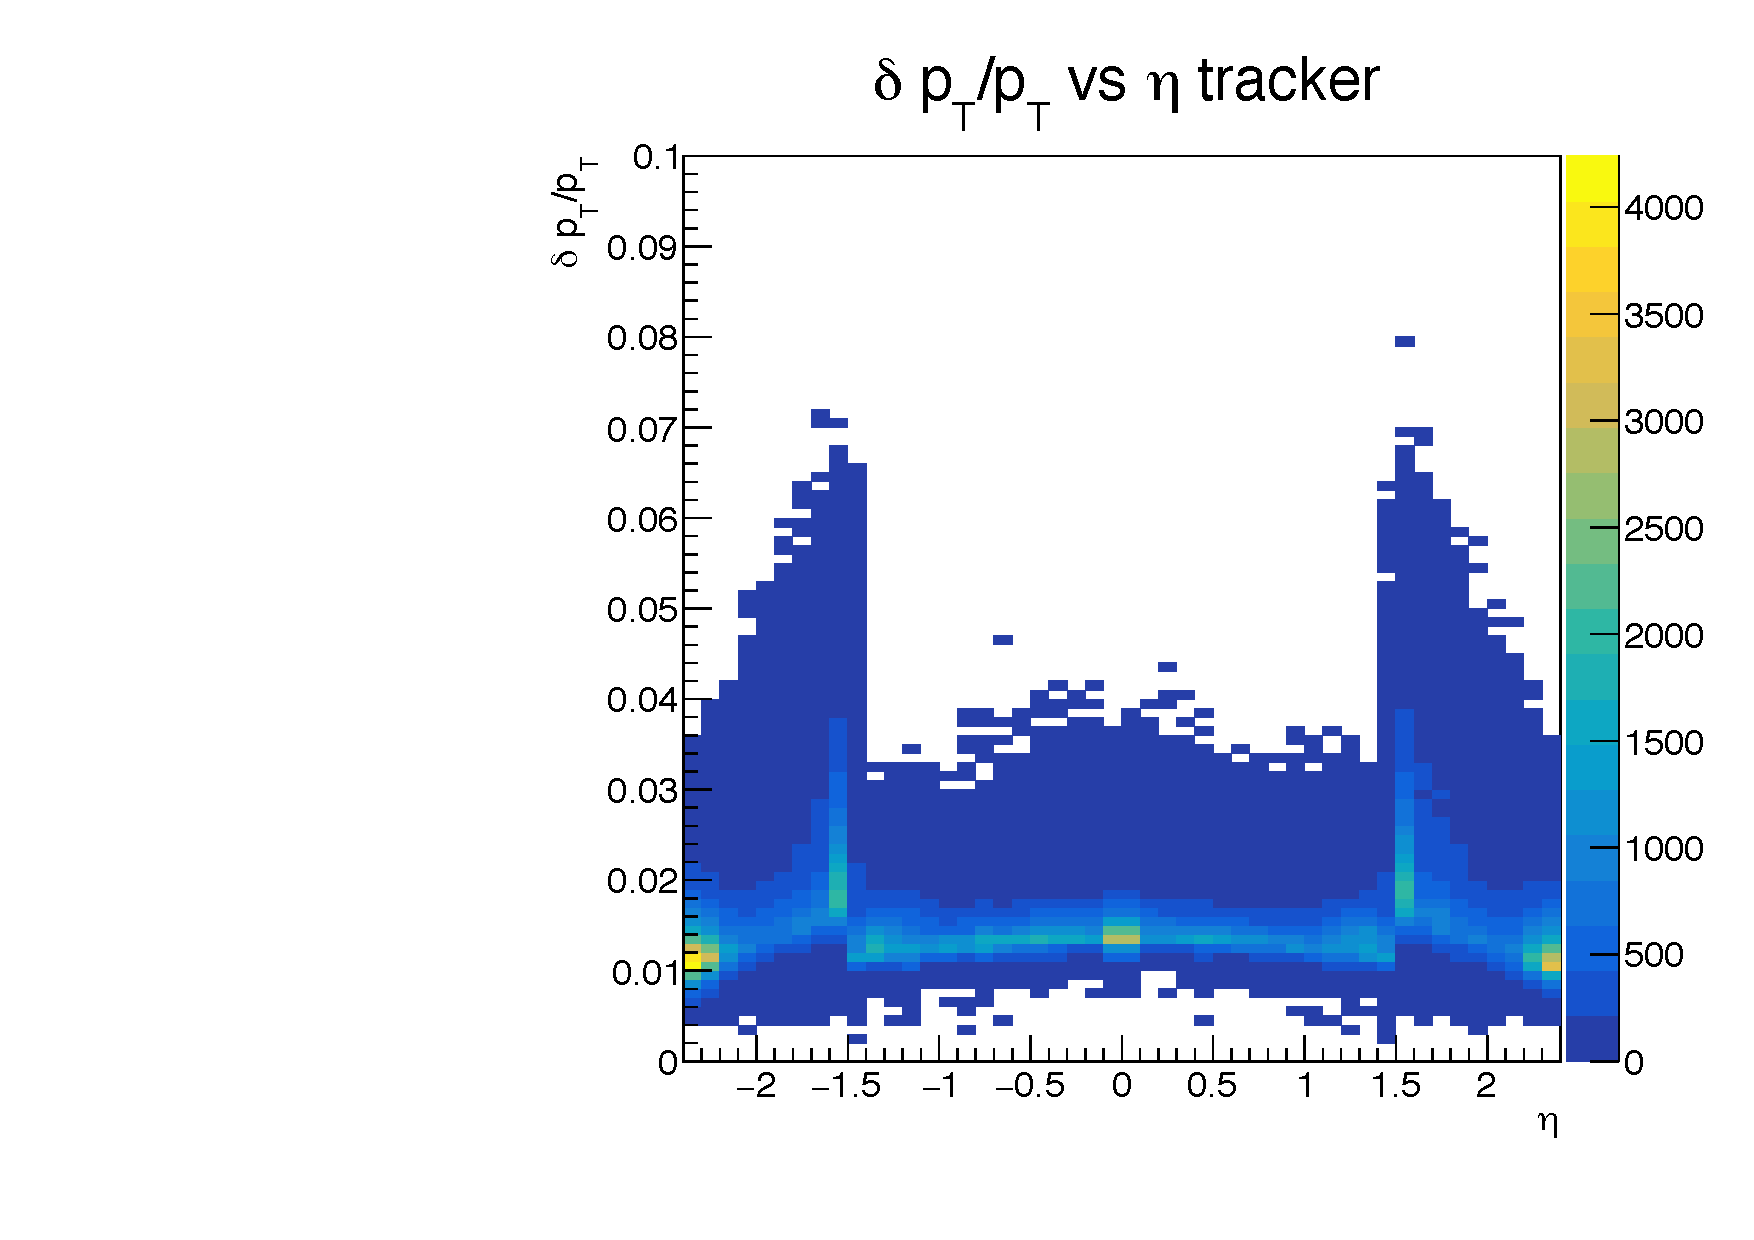
\includegraphics[width=0.32\textwidth]{Figures/EBE/2016_vs_eta_ele_tracker.pdf}
% %			}\\
% %		\subfloat[][2017]
%             % {
% 		    		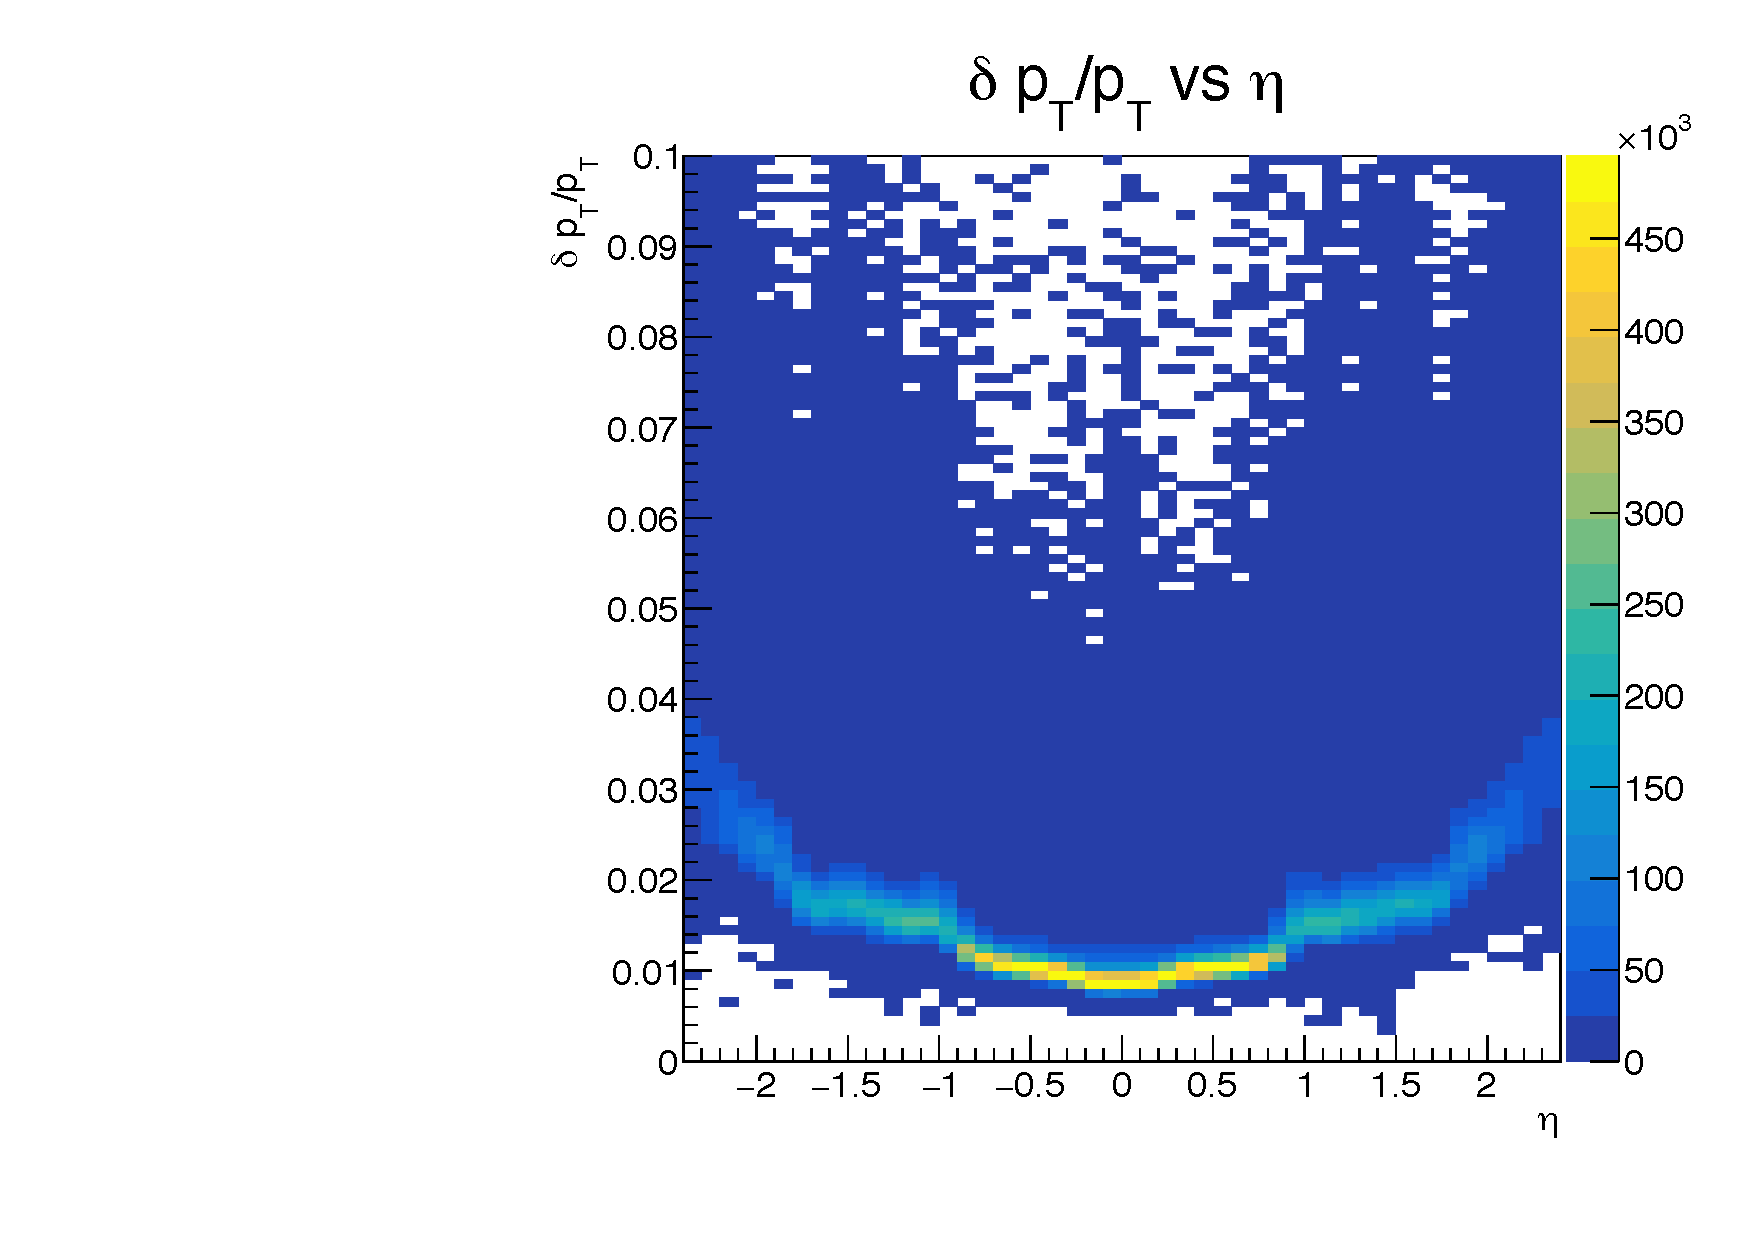
\includegraphics[width=0.32\textwidth]{Figures/EBE/2017_vs_eta_muon.pdf}
% 					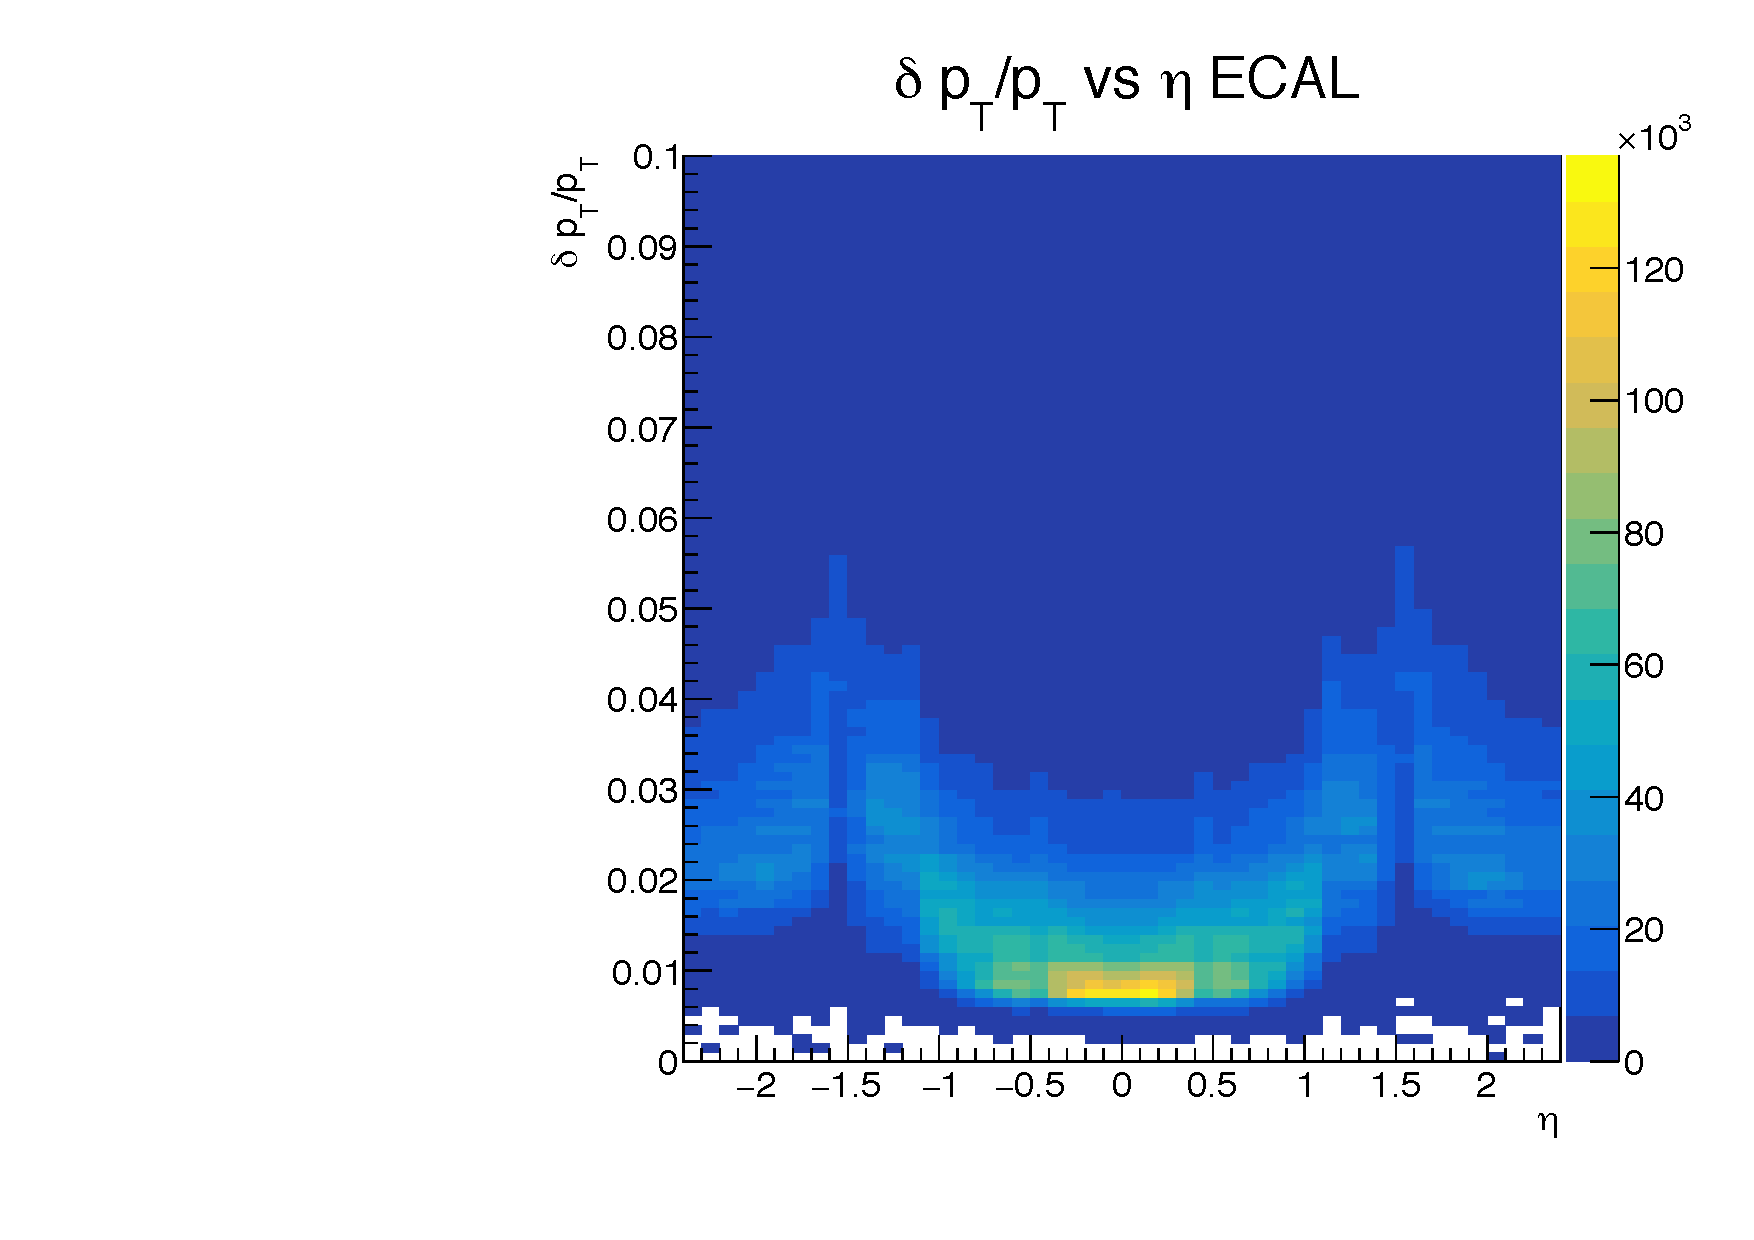
\includegraphics[width=0.32\textwidth]{Figures/EBE/2017_vs_eta_ele_ECAL.pdf} 
% 					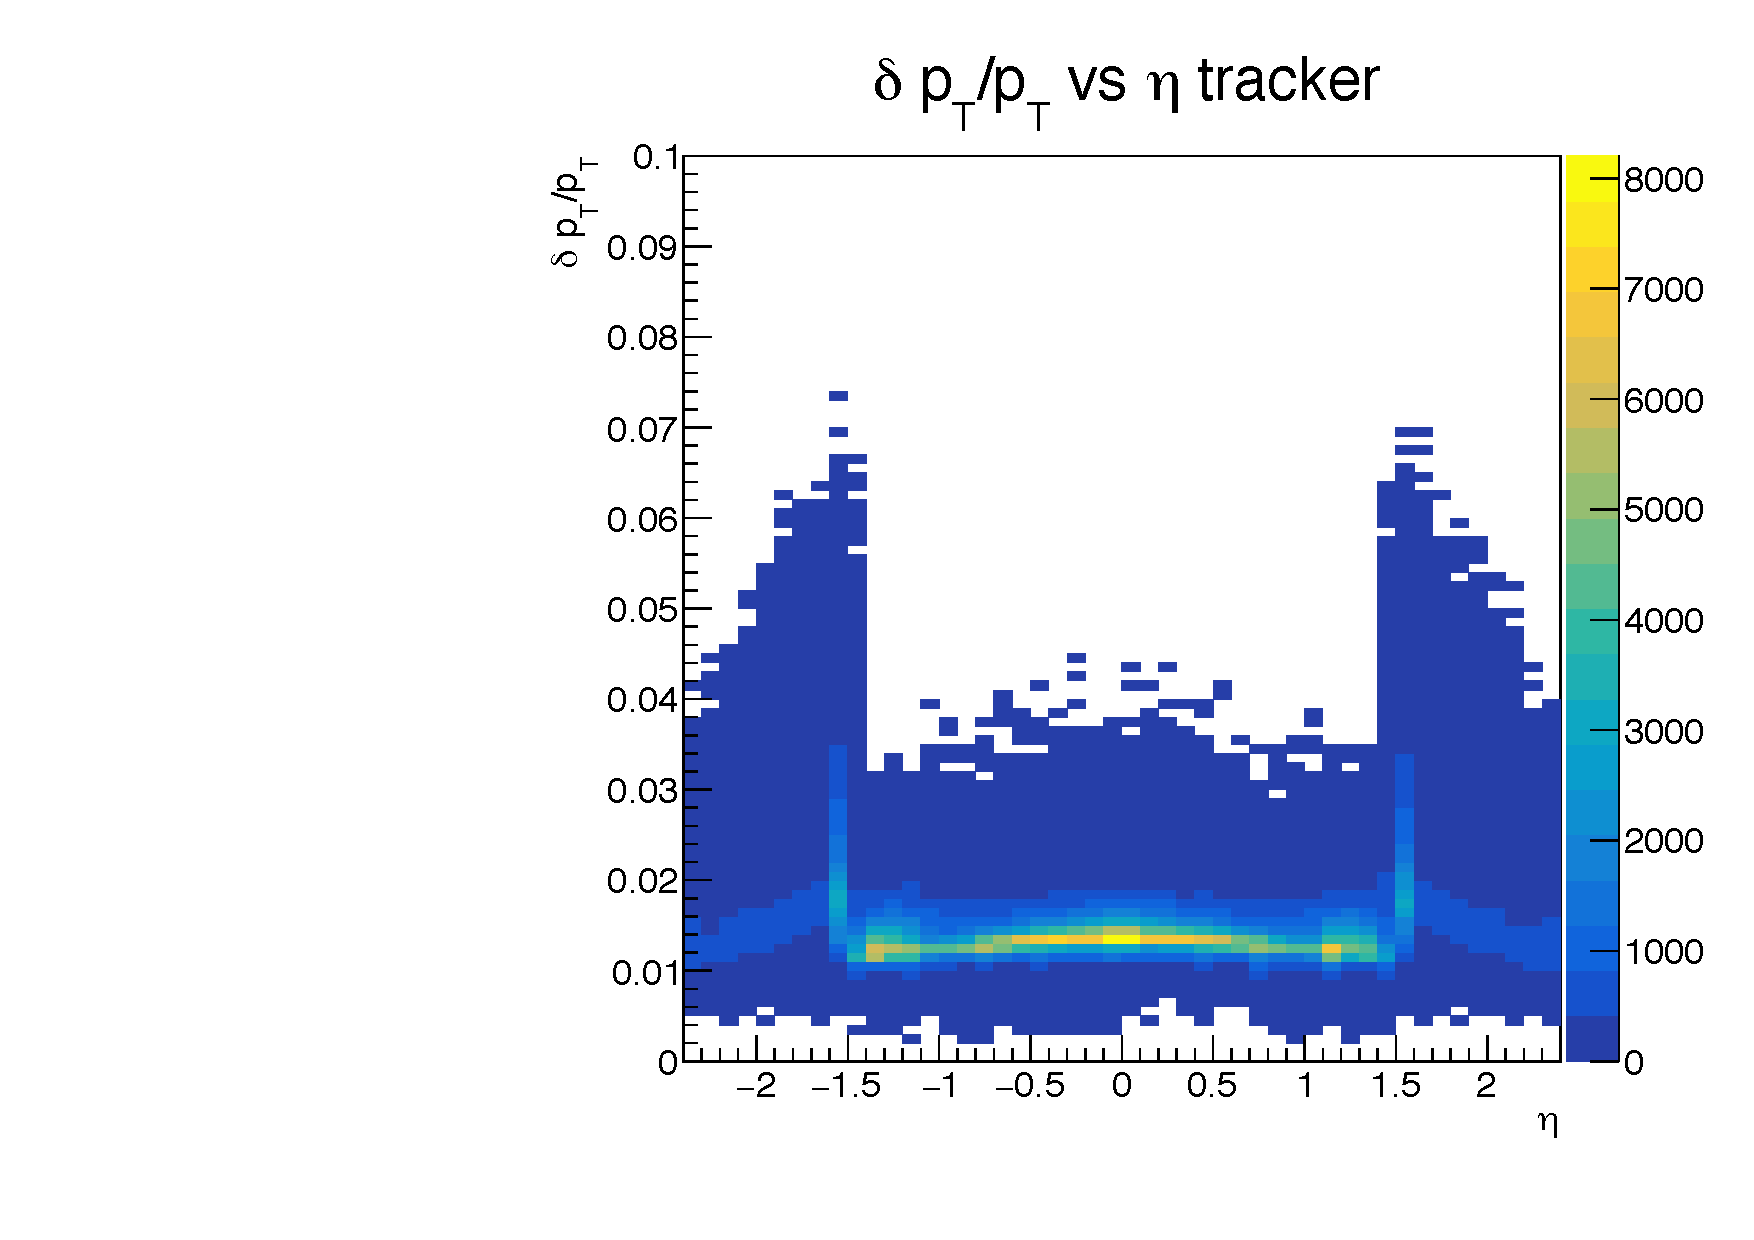
\includegraphics[width=0.32\textwidth]{Figures/EBE/2017_vs_eta_ele_tracker.pdf}
% %			}\\
% %		\subfloat[][2018]
%             % {
% 		    		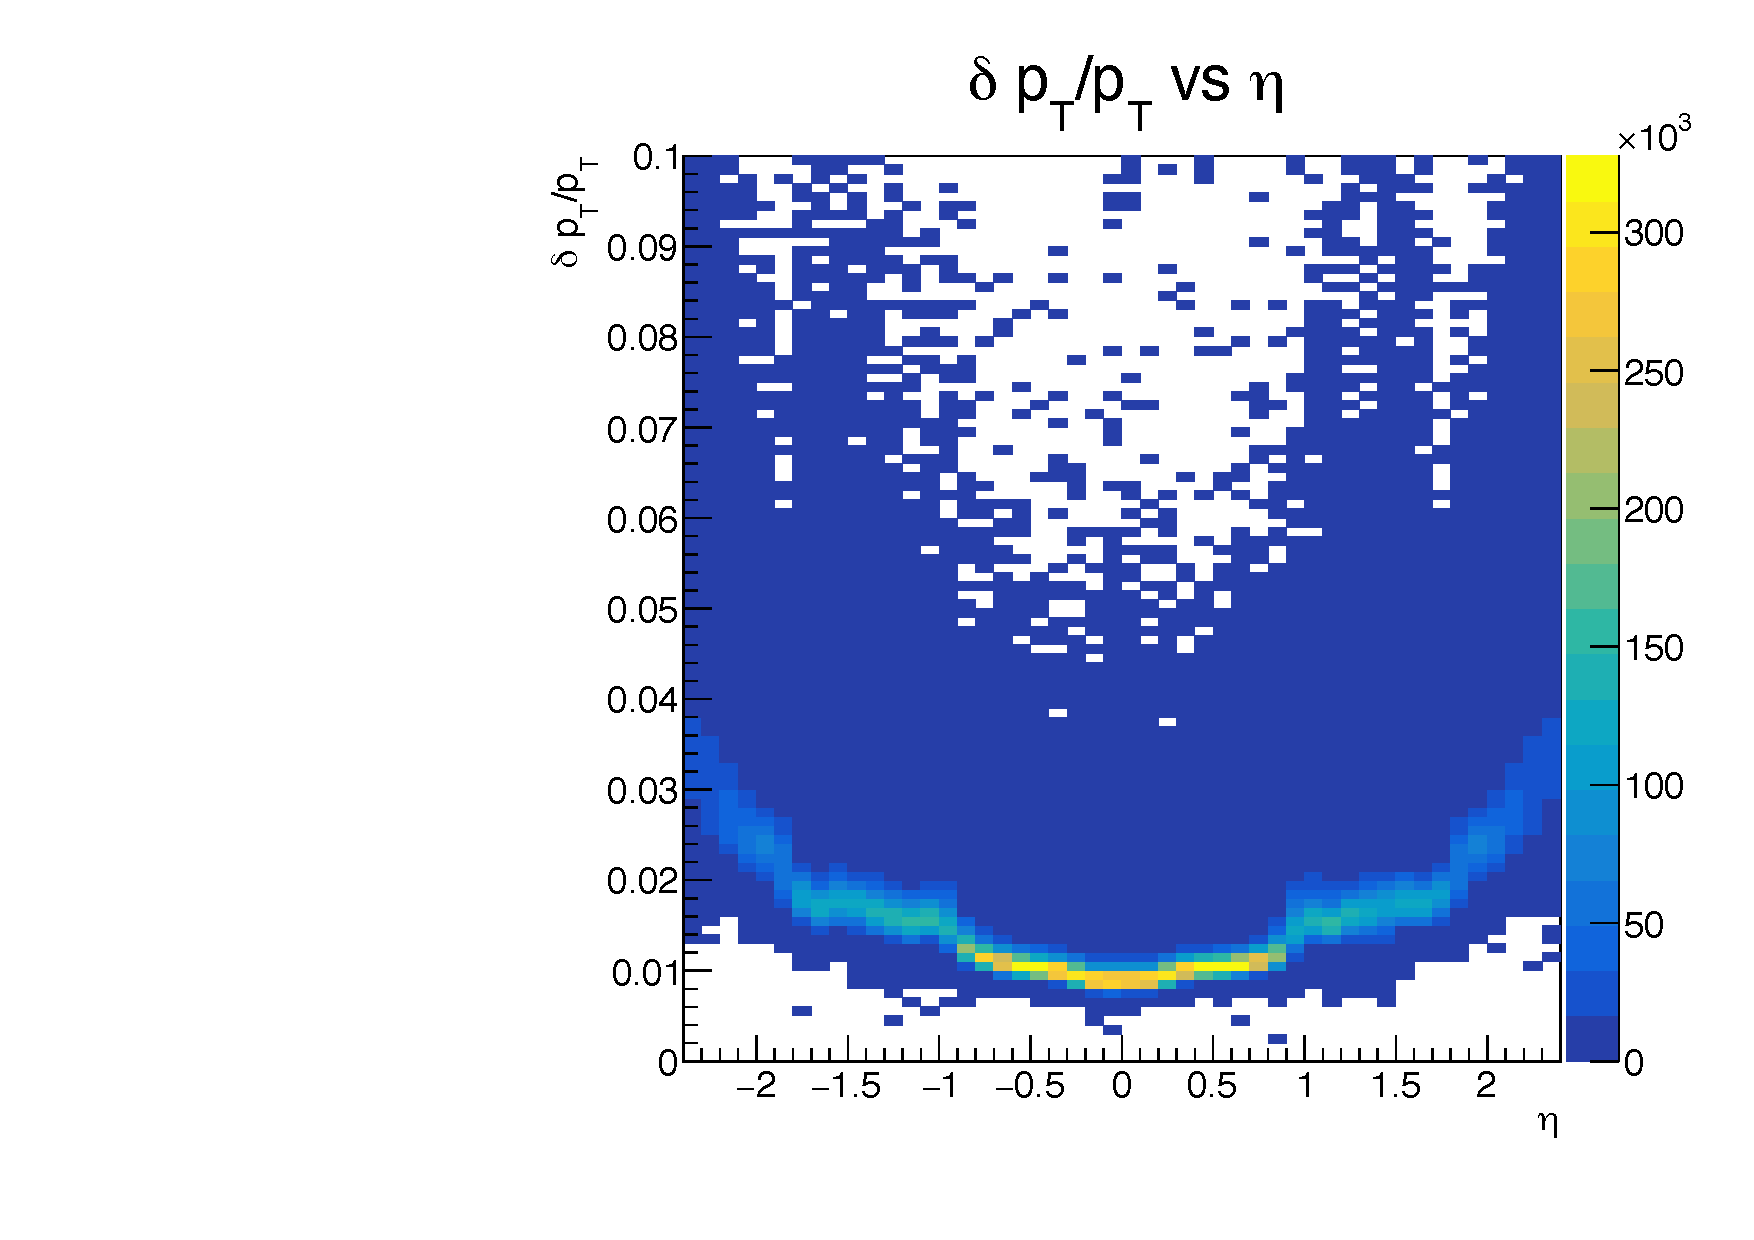
\includegraphics[width=0.32\textwidth]{figures/higgsmassmeas/ebe/2018_vs_eta_muon.pdf}
% 					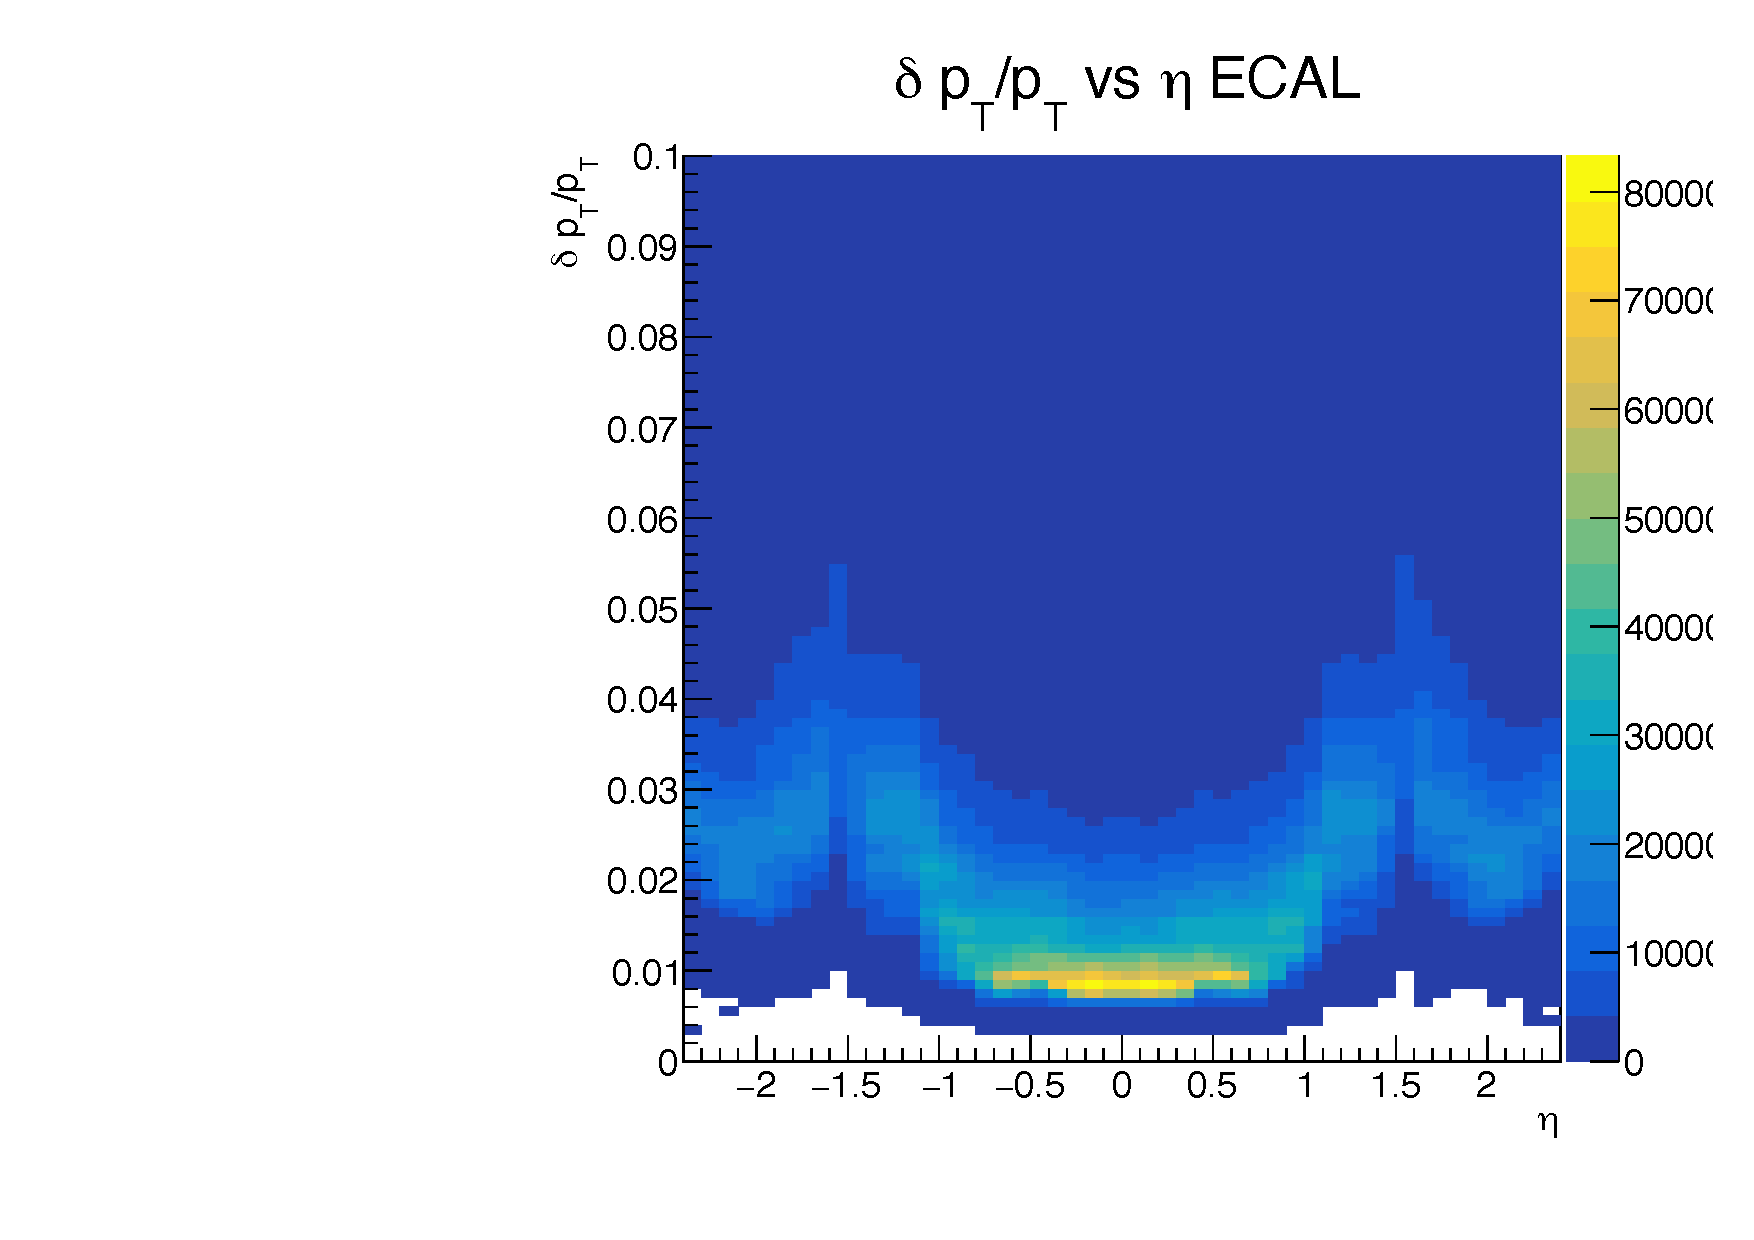
\includegraphics[width=0.32\textwidth]{figures/higgsmassmeas/ebe/2018_vs_eta_ele_ECAL.pdf} 
% 					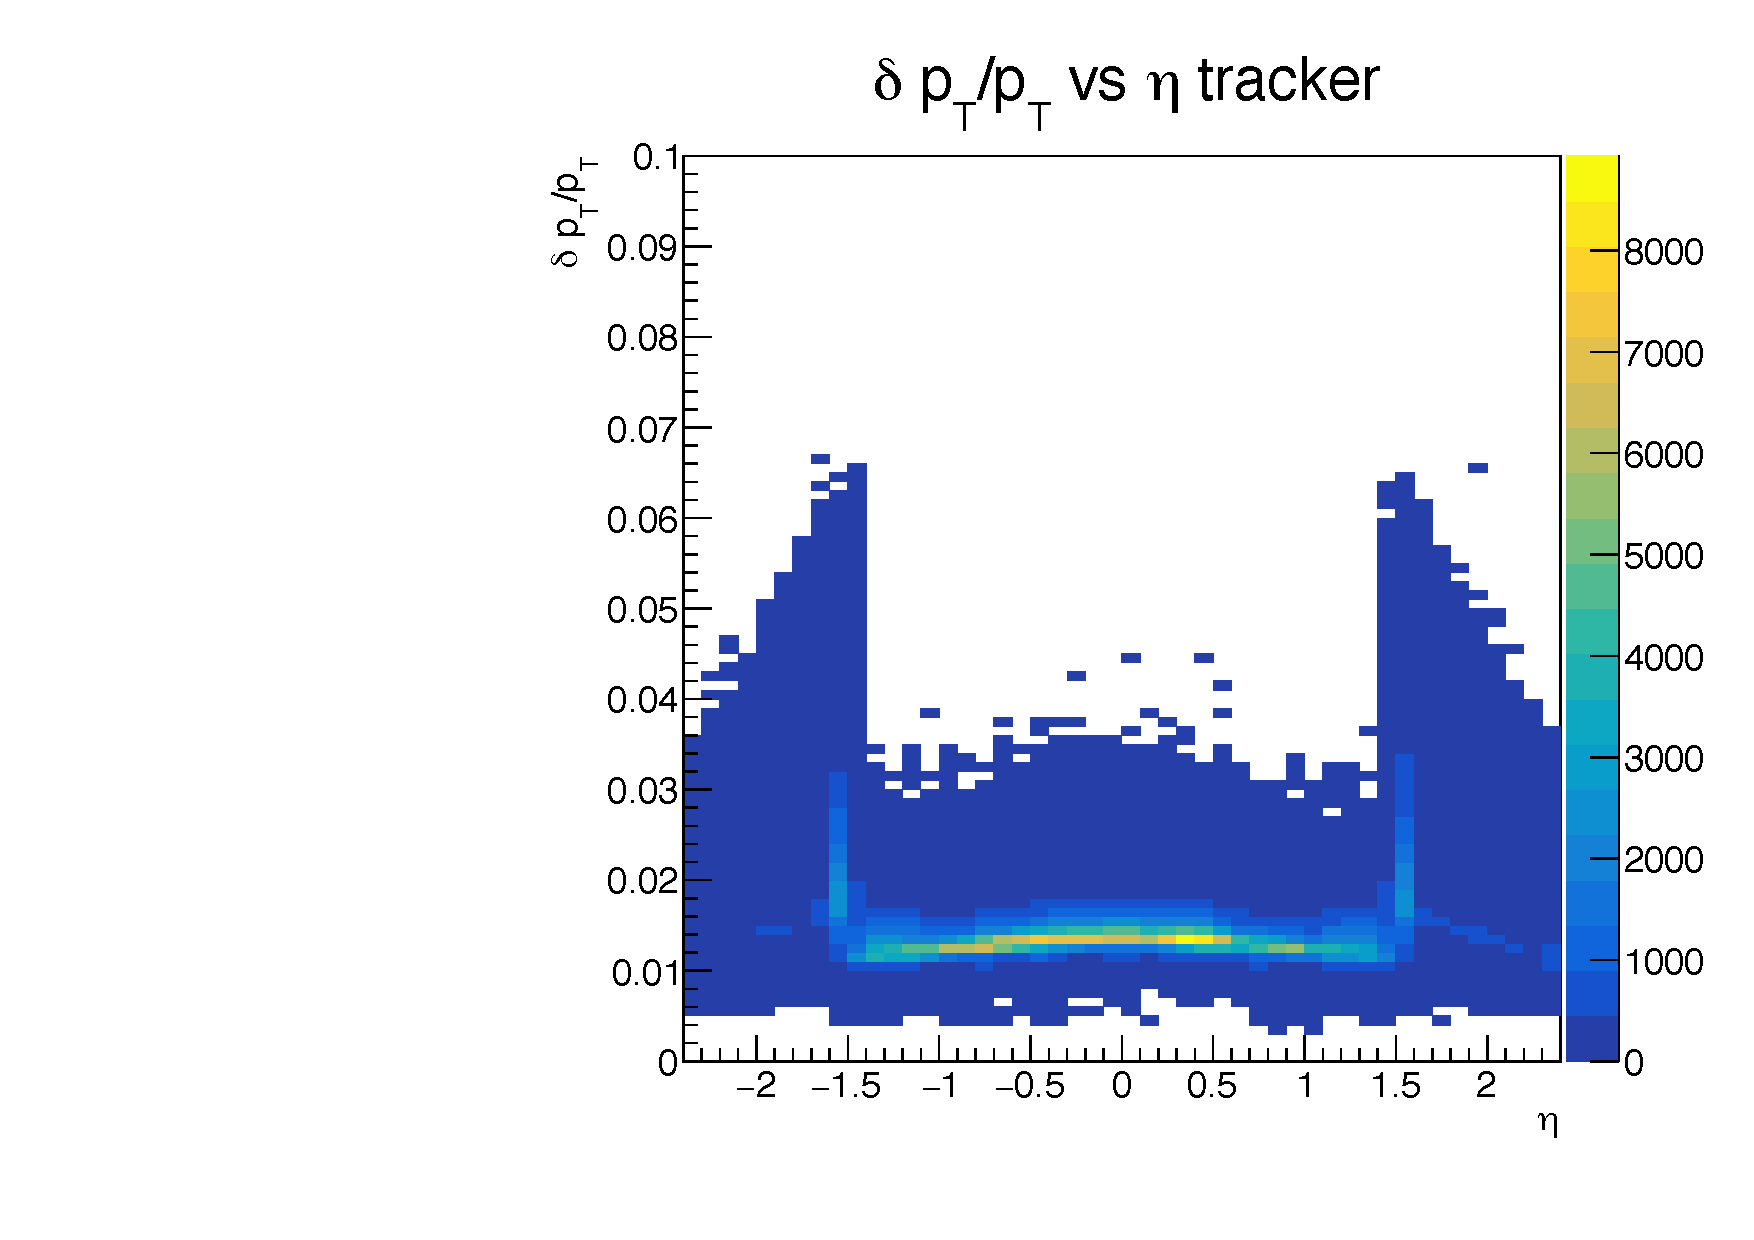
\includegraphics[width=0.32\textwidth]{figures/higgsmassmeas/ebe/2018_vs_eta_ele_tracker.pdf}
% %			}\\
% 		\caption{Scatterplot of the relative lepton \PT error vs $\eta$ for muons (left), 
% 				ECAL driven electrons (middle), and tracker driven electrons (right) for 2018 data.}
% 	\label{fig:2D_Mpas_vs_eta}
% 	\end{center}
% \end{figure}

Starting from these distributions, corrections to lepton momentum uncertainty in mutual $|\eta|$ bins are derived for muons (Fig.~\ref{fig:2D_Mpas_vs_pt_muon}), ECAL-driven electrons (Fig.~\ref{fig:2D_Mpas_vs_pt_electron_ECAL}), and tracker electrons (Fig.~\ref{fig:2D_Mpas_vs_pt_electron_tracker}) using bins of $\delta p_{T}$/$p_{T}$ \vs \abseta.
Scatterplots of $\delta p_{T}$/$p_{T}$ \vs \PT are shown in Figs.~\ref{fig:2D_Mpas_vs_pt_electron_ECAL} and~\ref{fig:2D_Mpas_vs_pt_electron_tracker}.
% Muons.
\begin{multiFigure}
    \centering
    \addFigure{0.32}{../../higgsmassmeasurement/AN-19-248/Figures/EBE/2016_vs_pt_muon_1_workinprogress.pdf}
    \addFigure{0.32}{../../higgsmassmeasurement/AN-19-248/Figures/EBE/2016_vs_pt_muon_2_workinprogress.pdf}
    \addFigure{0.32}{../../higgsmassmeasurement/AN-19-248/Figures/EBE/2016_vs_pt_muon_3_workinprogress.pdf}

    \addFigure{0.32}{../../higgsmassmeasurement/AN-19-248/Figures/EBE/2017_vs_pt_muon_1_workinprogress.pdf}
    \addFigure{0.32}{../../higgsmassmeasurement/AN-19-248/Figures/EBE/2017_vs_pt_muon_2_workinprogress.pdf}
    \addFigure{0.32}{../../higgsmassmeasurement/AN-19-248/Figures/EBE/2017_vs_pt_muon_3_workinprogress.pdf}

    \addFigure{0.32}{../../higgsmassmeasurement/AN-19-248/Figures/EBE/2018_vs_pt_muon_1_workinprogress.pdf}
    \addFigure{0.32}{../../higgsmassmeasurement/AN-19-248/Figures/EBE/2018_vs_pt_muon_2_workinprogress.pdf}
    \addFigure{0.32}{../../higgsmassmeasurement/AN-19-248/Figures/EBE/2018_vs_pt_muon_3_workinprogress.pdf}
    \captionof{figure}
        [Scatterplots of the relative \pT error vs \pT for muons in bins of \abseta]
        % TODO: fix words below.
        {Scatterplots of the relative \pT error vs \pT for muons. $0 < \abseta < 0.9$ (left column), $0.9 < \abseta < 1.8$ (middle column), and $1.8 < \abseta < 2.4$ (right column) for 2016 (top row), 2017 (middle row), and 2018 (bottom row) data.}
    \label{fig:2D_Mpas_vs_pt_muon}
\end{multiFigure}
% ECAL electrons.
\begin{multiFigure}
    \centering
    \addFigure{0.32}{../../higgsmassmeasurement/AN-19-248/Figures/EBE/2016_vs_pt_ECAL_1_workinprogress.pdf}
    \addFigure{0.32}{../../higgsmassmeasurement/AN-19-248/Figures/EBE/2016_vs_pt_ECAL_2_workinprogress.pdf}
    \addFigure{0.32}{../../higgsmassmeasurement/AN-19-248/Figures/EBE/2016_vs_pt_ECAL_3_workinprogress.pdf}

    \addFigure{0.32}{../../higgsmassmeasurement/AN-19-248/Figures/EBE/2017_vs_pt_ECAL_1_workinprogress.pdf}
    \addFigure{0.32}{../../higgsmassmeasurement/AN-19-248/Figures/EBE/2017_vs_pt_ECAL_2_workinprogress.pdf}
    \addFigure{0.32}{../../higgsmassmeasurement/AN-19-248/Figures/EBE/2017_vs_pt_ECAL_3_workinprogress.pdf}

    \addFigure{0.32}{../../higgsmassmeasurement/AN-19-248/Figures/EBE/2018_vs_pt_ECAL_1_workinprogress.pdf}
    \addFigure{0.32}{../../higgsmassmeasurement/AN-19-248/Figures/EBE/2018_vs_pt_ECAL_2_workinprogress.pdf}
    \addFigure{0.32}{../../higgsmassmeasurement/AN-19-248/Figures/EBE/2018_vs_pt_ECAL_3_workinprogress.pdf}
    \captionof{figure}
        [Scatterplots of the relative \pT error vs \pT for ECAL-driven electrons in bins of \abseta]
        % TODO: Is it OK to skip over 1.0--2.0?
        {Scatterplots of the relative \pT error vs \pT for ECAL-driven electrons with $0 < \abseta < 0.8$ (left column), $0.8 < \abseta < 1.0$ (middle column), and $2.0 < \abseta < 2.5$ (right column) for 2016 (top row), 2017 (middle row), and 2018 (bottom row) data.}
    \label{fig:2D_Mpas_vs_pt_electron_ECAL}
\end{multiFigure}
% Tracker electrons.
\begin{multiFigure}
    \centering
    \addFigure{0.32}{../../higgsmassmeasurement/AN-19-248/Figures/EBE/2016_vs_pt_tracker_1_workinprogress.pdf}
    \addFigure{0.32}{../../higgsmassmeasurement/AN-19-248/Figures/EBE/2016_vs_pt_tracker_2_workinprogress.pdf}
    \addFigure{0.32}{../../higgsmassmeasurement/AN-19-248/Figures/EBE/2016_vs_pt_tracker_3_workinprogress.pdf}

    \addFigure{0.32}{../../higgsmassmeasurement/AN-19-248/Figures/EBE/2017_vs_pt_tracker_1_workinprogress.pdf}
    \addFigure{0.32}{../../higgsmassmeasurement/AN-19-248/Figures/EBE/2017_vs_pt_tracker_2_workinprogress.pdf}
    \addFigure{0.32}{../../higgsmassmeasurement/AN-19-248/Figures/EBE/2017_vs_pt_tracker_3_workinprogress.pdf}

    \addFigure{0.32}{../../higgsmassmeasurement/AN-19-248/Figures/EBE/2018_vs_pt_tracker_1_workinprogress.pdf}
    \addFigure{0.32}{../../higgsmassmeasurement/AN-19-248/Figures/EBE/2018_vs_pt_tracker_2_workinprogress.pdf}
    \addFigure{0.32}{../../higgsmassmeasurement/AN-19-248/Figures/EBE/2018_vs_pt_tracker_3_workinprogress.pdf}
    \captionof{figure}
        [Scatterplots of the relative lepton \PT error \vs \PT for tracker-driven electrons]
        % TODO: Is it OK to skip over 1.44--1.6?
        {Scatterplots of the relative lepton \PT error \vs \PT for tracker-driven electrons with $0 < \abseta < 0.8$ (left column), $1.0 < \abseta < 1.44$ (middle column), and $1.6 < \abseta < 2.0$ (right column) for 2016 (top row), 2017 (middle row), and 2018 (bottom row) data.}
    \label{fig:2D_Mpas_vs_pt_electron_tracker}
\end{multiFigure}

\subsubsection{Procedure to Derive Corrections to $\delta \ptl$}
% TODO: REWORD
To derive the corrections ($\lambda$), the dilepton invariant mass $\left( \mll \right)$ from \ztolplm events is fitted twice with a Breit--Wigner (BW) function convolved with a Crystal Ball (CB), plus an exponential function (EXP).
In this model, the BW represents the true \mZ lineshape, the CB simulates the detector effects, and the EXP describes the falling background.
When deriving the corrections, the mean and sigma of the BW have been set to the PDG values $\left( \mZ = 91.19\GeV, \; \Gamma_{\PZ} = 2.49\GeV \right)$~\cite{particle_data_group_review_2020}.
 The fit is done in the mass range [60, 120]\GeV, using only
$e^{+}e^{-}$ or $\mu^{+}\mu^{-}$ pairs.\\
The first fit is used to fix all the parameters of the functions but the $\sigma$ of the CB which is
replaced in the second fit by $\lambda$ $\times$ $\delta_{m_{Z}}$, where $\lambda$ is the 
floated parameter of the fit. 

The summary of $\lambda$ correction factors for electrons and muons is shown in Table~\ref{table:Lambdas}.
\begin{table}[!h]\fontsize{10}{12}\selectfont
    \topcaption
        [Event-by-event lambda correction factors.] % TODO: reword
        {Event-by-event lambda correction factors.}
    \begin{tabularx}{\textwidth}{BMSSSSSSSS} % TODO: Fix  numbers in table.
        \toprule 
        \multicolumn{2}{c}{\textbf{2016 pre-VFP}} & \multicolumn{2}{c}{\textbf{2016 post-VFP}} & \multicolumn{2}{c}{\textbf{2017}} & \multicolumn{2}{c}{\textbf{2018}} \\ \toprule

        && \multicolumn{8}{c}{Muons} \\
        \multicolumn{2}{c}{$0 < |\eta| < 0.9$} & 1.05 & 1.248 & 1.043 & 1.214 & 1.047 & 1.183 & 1.019 & 1.227 \\
        \multicolumn{2}{c}{$0.9 < |\eta| < 1.8$} & 1.187 & 1.256 & 1.204 & 1.234 & 1.219 & 1.223 & 1.206 & 1.236 \\
        \multicolumn{2}{c}{$1.8 < |\eta| < 2.4$} & 1.197 & 1.201 & 1.183 & 1.164 & 1.197 & 1.173 & 1.108 & 1.188 \\ \toprule

        && \multicolumn{8}{c}{ECAL electrons} \\ 
        $0 < |\eta| < 0.8$ & $\delta p_T/p_T < 0.01$ & 1.648 & 1.619 & 1.645 & 1.646 & 1.690 & 1.633 & 1.676 & 1.661 \\
        $0 < |\eta| < 0.8$ & $0.01 < \delta p_T/p_T < 0.015$ & 1.490 & 1.506 & 1.470 & 1.528 & 1.540 & 1.496 & 1.544 & 1.511 \\
        $0 < |\eta| < 0.8$ & $0.015 < \delta p_T/p_T < 0.025$ & 1.490 & 1.506 & 1.470 & 1.528 & 1.540 & 1.496 & 1.544 & 1.511 \\
        $0 < |\eta| < 1$ & $0.025 < \delta p_T/p_T < 1$ & 1.490 & 1.506 & 1.470 & 1.528 & 1.540 & 1.496 & 1.544 & 1.511 \\
        $1 < |\eta| < 2.5$ & $\delta p_T/p_T < 0.02$ & 1.490 & 1.506 & 1.470 & 1.528 & 1.540 & 1.496 & 1.544 & 1.511 \\
        $1 < |\eta| < 2.5$ & $0.03 < \delta p_T/p_T < 0.04$ & 1.490 & 1.506 & 1.470 & 1.528 & 1.540 & 1.496 & 1.544 & 1.511 \\
        $1 < |\eta| < 2.5$ & $0.04 < \delta p_T/p_T < 0.05$ & 1.490 & 1.506 & 1.470 & 1.528 & 1.540 & 1.496 & 1.544 & 1.511 \\
        $1 < |\eta| < 2.5$ & $0.05 < \delta p_T/p_T < 0.06$ & 1.490 & 1.506 & 1.470 & 1.528 & 1.540 & 1.496 & 1.544 & 1.511 \\
        $0.8 < |\eta| < 2.5$ & $\delta p_T/p_T < 0.025$ & 1.490 & 1.506 & 1.470 & 1.528 & 1.540 & 1.496 & 1.544 & 1.511 \\
        $1 < |\eta| < 2.5$ & $0.06 < \delta p_T/p_T < 1$ & 1.490 & 1.506 & 1.470 & 1.528 & 1.540 & 1.496 & 1.544 & 1.511 \\ \toprule
        
        && \multicolumn{8}{c}{Tracker electrons} \\ 
        \multicolumn{2}{c}{$0 < |\eta| < 1.44$} & 1.05 & 1.248 & 1.043 & 1.214 & 1.047 & 1.183 & 1.019 & 1.227 \\
        \multicolumn{2}{c}{$1.44 < |\eta| < 1.6$} & 1.187 & 1.256 & 1.204 & 1.234 & 1.219 & 1.223 & 1.206 & 1.236 \\
        \multicolumn{2}{c}{$1.6 < |\eta| < 2$} & 1.197 & 1.201 & 1.183 & 1.164 & 1.197 & 1.173 & 1.108 & 1.188 \\
        \multicolumn{2}{c}{$2 < |\eta| < 2.5$} & 1.197 & 1.201 & 1.183 & 1.164 & 1.197 & 1.173 & 1.108 & 1.188 \\ \hline
    \end{tabularx}
    \label{table:Lambdas}
\end{table}

% \begin{table}[ht]	
% 	\begin{center}
% 		\begin{tabular}{ccccccc}
% 			\hline
% 			\hline			
% 			& \multicolumn{2}{c}{\textbf{2016}} & \multicolumn{2}{c}{\textbf{2017}} & \multicolumn{2}{c}{\textbf{2018}} \\
% 			& \multicolumn{1}{c}{\textbf{MC}} & \multicolumn{1}{c}{\textbf{Data}} & \multicolumn{1}{c}{\textbf{MC}} & \multicolumn{1}{c}{\textbf{Data}} & \multicolumn{1}{c}{\textbf{MC}} & \multicolumn{1}{c}{\textbf{Data}} \\
% 			\hline
% 			\hline
% 			& \multicolumn{6}{c}{Muons} \\
% 			$ 0 < |\eta| < 0.9$ &	1.05	&	1.248	&	1.043	&	1.214	&	1.047		&	1.183	&	1.019	&	1.227	\\
%                        $ 0.9 < |\eta| < 1.8$ &	1.187	&	1.256	&	1.204	&	1.234	&	1.219	&	1.223	&	1.206	&	1.236	\\
%                        $ 1.8 < |\eta| < 2.4$ &	1.197	&	1.201	&	1.183	&	1.164	&	1.197	&	1.173	&	1.108	&	1.188	\\
% 			\hline
% 			\hline
% 			& \multicolumn{6}{c}{ECAL electrons} \\
% 			$0 < |\eta| < 0.8$ and $\delta\pt/\pt < 0.01$            & 2.006 & 1.893 & 2.086 & 2.030 & 2.054 & 1.914 \\
%                        $0 < |\eta| < 0.8$ and $0.01 < \delta\pt/\pt < 0.015$    & 1.590 & 1.575 & 1.698 & 1.680 & 1.701 & 1.635\\
%                        $0 < |\eta| < 0.8$ and $0.015 < \delta\pt/\pt < 0.025$   & 1.406 & 1.373 & 1.426 & 1.450 & 1.447 & 1.467\\
%                        $0 < |\eta| < 1$ and $0.025 < \delta\pt/\pt < 1$         & 1.517 & 1.531 & 1.481 & 1.521 & 1.560 & 1.569\\
%                        $1 < |\eta| < 2.5$ and $\delta\pt/\pt < 0.02$            & 2.116 & 2.002 & 2.305 & 2.210 & 2.324 & 2.228\\
%                        $1 < |\eta| < 2.5$ and $0.02 < \delta\pt/\pt < 0.03$     & 1.645 & 1.623 & 1.815 & 1.795 & 1.787 & 1.759\\
%                        $1 < |\eta| < 2.5$ and $0.03 < \delta\pt/\pt < 0.04$     & 1.472 & 1.489 & 1.568 & 1.560 & 1.468 & 1.509\\
%                        $1 < |\eta| < 2.5$ and $0.04 < \delta\pt/\pt < 0.06$     & 1.374 & 1.448 & 1.414 & 1.606 & 1.378 & 1.477\\
%                        $0.8 < |\eta| < 1$ and $\delta\pt/\pt < 0.025$           & 1.149 & 1.203 & 1.196 & 1.241 & 1.180 & 1.286\\
%                        $1 < |\eta| < 2.5$ and $0.06 < \delta\pt/\pt < 1$        & 1.099 & 1.221 & 1.171 & 1.331 & 1.123 & 1.272\\
% 			\hline
% 			\hline
% 			& \multicolumn{6}{c}{tracker electrons} \\
% 			$0 < |\eta| < 1.44$ & 1.619 & 1.872 & 2.382 & 2.115 & 2.120 & 1.936\\
%                        $1.44 < |\eta| < 1.6$ & 6.452 & 5.900 & 6.572 & 7.056 & 5.613 & 5.524\\
%                        $1.6 < |\eta| < 2$ & 2.732 & 2.826 & 3.430 &2.846& 3.204 & 3.016\\
%                        $2 < |\eta| <2.5$ & 3.010 &3.081& 3.963 &3.817& 4.110 & 3.762\\
% 			\hline
% 		\end{tabular}
% 	\end{center}
% 	\caption{\PT error corrections for muons and electrons in different kinematic region. For each year, MC 
% 	is on the left, data on the right.}
% 	\label{table:Lambdas}
% \end{table}
% TODO: Figure 8 (from AN) of lambdas vs. dpT/pT bins? CONTAINS DATA.

% TODO: REWORD.
\subsubsection{Validation of corrections (MC, data)}
\label{sec:ClosureTest}
A closure test is performed to validate correction derived for lepton \PT error. \\
First, events are divided according to different predicted $\delta m_{Z}/m_{Z}$ ranges before corection. 
Then, in each bin, the dilepton invariant mass distribution is fitted using a BW convoluted with CB 
plus exponential function, to get $\delta m_{Z}^{fit}$ (measured $m_{Z}$ resolution). Finally 
the average predicted $\delta m_{Z}$ is calculated in each $\delta m_{Z}/m_{Z}$ bin before and after the 
correction factor for lepton \PT error is applied (predicted $m_{Z}$ resolution). \\
In the closure plot, it is expected to see $\delta m_{Z}$ gets closer to $\delta m_{Z}^{fit}$ 
after correction, and the points should stay in a band which is 20\% around diagonal line, which 
is the uncertainty assigned to the resolution in the previous analysis \cite{HIG_16_041}. 
This closure test is shown in Fig.~\ref{fig:ZClosure_test_MU} for muons and in Fig.~\ref{fig:ZClosure_test_ELE} 
for electrons. A further check has been also performed, looking at the closure test of the predicted four lepton mass 
resolution compared to the fitted four lepton mass resolution using H signal MC samples once the 
corrections derived using \PZ events are applied. After applying corrections, measured $m_{4l}$ 
resolution gets closer to the prediction. This closure test is shown for three different 
final states in Fig.~\ref{fig:HClosure_test}.
% CLOSURE: Z->mumu MC.
\begin{multiFigure}
    \centering
    \addFigure{0.45}{../../higgsmassmeasurement/AN-19-248/Figures/EBE/VXBS_20160_MC_workinprogress.pdf}
    \addFigure{0.45}{../../higgsmassmeasurement/AN-19-248/Figures/EBE/VXBS_20165_MC_workinprogress.pdf}
    \addFigure{0.45}{../../higgsmassmeasurement/AN-19-248/Figures/EBE/VXBS_2017_MC_workinprogress.pdf}
    \addFigure{0.45}{../../higgsmassmeasurement/AN-19-248/Figures/EBE/VXBS_2018_MC_workinprogress.pdf}
    \captionof{figure}
        % [Closure plots showing corrections to lepton momentum uncertainty on \ztomumu events]
        [Validation of the per-event mass uncertainties from simulated \ztomumu events]
        {Validation of the per-event mass uncertainties from simulated \ztomumu events.
        The solid blue line corresponds to a 10\% band relative to the solid green 1:1 line.
        \;A) 2016 pre-VFP.
        \;B) 2016 post-VFP.
        \;C) 2017.
        \;D) 2018.
		}
    \label{fig:ZClosure_test_MU}
\end{multiFigure}
% CLOSURE: Z->ee MC.
\begin{multiFigure}
    \centering
    \addFigure{0.45}{../../higgsmassmeasurement/AN-19-248/Figures/EBE/ZEE_20160_MC_workinprogress.pdf}
    \addFigure{0.45}{../../higgsmassmeasurement/AN-19-248/Figures/EBE/ZEE_20165_MC_workinprogress.pdf}
    \addFigure{0.45}{../../higgsmassmeasurement/AN-19-248/Figures/EBE/ZEE_2017_MC_workinprogress.pdf}
    \addFigure{0.45}{../../higgsmassmeasurement/AN-19-248/Figures/EBE/ZEE_2018_MC_workinprogress.pdf}
    \captionof{figure}
        [Validation of the per-event mass uncertainties using simulated \ztoee events]
        {Validation of the per-event mass uncertainties using simulated \ztoee events.
        The solid blue line corresponds to a 10\% band relative to the solid green 1:1 line.
        \;A) 2016 pre-VFP.
        \;B) 2016 post-VFP.
        \;C) 2017.
        \;D) 2018.
        }
    \label{fig:ZClosure_test_ELE}
\end{multiFigure}
% CLOSURE: ggH4l MC.
% $\sigma_\text{m}^\text{2e2\Pmu}\;(\GeVns)$ % FOR TESTING. DELETE
\begin{multiFigure}
    \centering
    \addFigure{0.32}{../../higgsmassmeasurement/AN-19-248/Figures/EBE/2016_H4mu_Closure_test_workinprogress.png}
    \addFigure{0.32}{../../higgsmassmeasurement/AN-19-248/Figures/EBE/2016_H4e_Closure_test_workinprogress.png}
    \addFigure{0.32}{../../higgsmassmeasurement/AN-19-248/Figures/EBE/2016_H2e2mu_Closure_test_workinprogress.png}

    \addFigure{0.32}{../../higgsmassmeasurement/AN-19-248/Figures/EBE/2017_H4mu_Closure_test_workinprogress.png}
    \addFigure{0.32}{../../higgsmassmeasurement/AN-19-248/Figures/EBE/2017_H4e_Closure_test_workinprogress.png}
    \addFigure{0.32}{../../higgsmassmeasurement/AN-19-248/Figures/EBE/2017_H2e2mu_Closure_test_workinprogress.png}
    
    \addFigure{0.32}{../../higgsmassmeasurement/AN-19-248/Figures/EBE/2018_H4mu_Closure_test_workinprogress.png}
    \addFigure{0.32}{../../higgsmassmeasurement/AN-19-248/Figures/EBE/2018_H4e_Closure_test_workinprogress.png}
    \addFigure{0.32}{../../higgsmassmeasurement/AN-19-248/Figures/EBE/2018_H2e2mu_Closure_test_workinprogress.png}
    \captionof{figure}
        [Validation of the per-event mass uncertainties using simulated \gghtofourl events]
        {Validation of the per-event mass uncertainties using simulated \gghtofourl events for
        2016 (top row), 2017 (middle row), and 2018 (bottom row) in three different final states:
		\fourmu (left column), \foure (middle column), and \twoetwomu (right column).
		The 20\% reference band is also shown.}
    \label{fig:HClosure_test}
\end{multiFigure}

\subsection{Vertex+Beamspot Constraint: VX+BS}
% \subsection{Methodology}
% so they all come from the primary vertex 
%interaction. \\
Leptons produced from the \hzzfourl channel should originate from the \pp collision point---the primary vertex---since the \PH boson and both \PZ bosons decay promptly after being formed.
% TODO: Explain why electrons are not given the vertex+beamspot constraint.
The primary vertex from which the muons originate can be approximated to come from the more general \emph{beamspot}, \ie the luminous region in the $x$-$y$ plane where the \pp bunches cross.
Thus, if the muon tracks are constrained to come from their vertex of origination ($\approx$beamspot), then one should expect a more accurate measurement of muon momentum and resolution.
The updated muon kinematical variables then get propagated into a more accurate estimate of the \mH value per event.
This process of constraining muon tracks to a vertex that is compatible with the beamspot is called the \emph{vertex+beamspot constraint} (VX+BS).

The pixel upgrade in the middle of Run 2 allowed for a more collimated (more precise) \pp beamspot.
Figure~\ref{fig:BeamY_vs_Y} shows the beamspot for 2018 Run D as compared to 2016 Run G.
Both the X and Y widths of the beamspot are smaller ($X_{2018} \approx 9 \mu m$ vs $X_{2016} \approx 14 \mu m$ and $Y_{2018} \approx 7 \mu m$ vs $Y_{2016} \approx 9 \mu m$), giving a better constraint when it is used in the track reconstruction.
% Beamspot information has been investigated in order to try to understand the reason why 2018 results have a two times better results.
% In Fig.~\ref{fig:BeamY_vs_Y}, the beamspot width (Y vs X) is shown for 2016 RunG and 2018 RunD.
% On the other hand, Fig.~\ref{fig:BeamXY_vs_Lumi} shows the width X and Y as a function of lumi section.
% As can be seen, in 2018, both X and Y widths of the beamspot are smaller ($X_{2018} \approx 9 \mu m$ vs $X_{2016} \approx 14 \mu m$ and $Y_{2018} \approx 7 \mu m$ vs $Y_{2016} \approx 9 \mu m$), letting a better constraint when it is used in the track reconstruction.
%=== Beamspot width Y vs. width X.
% TODO: Cut this picture up and do it properly?
\begin{multiFigure}
    \centering
        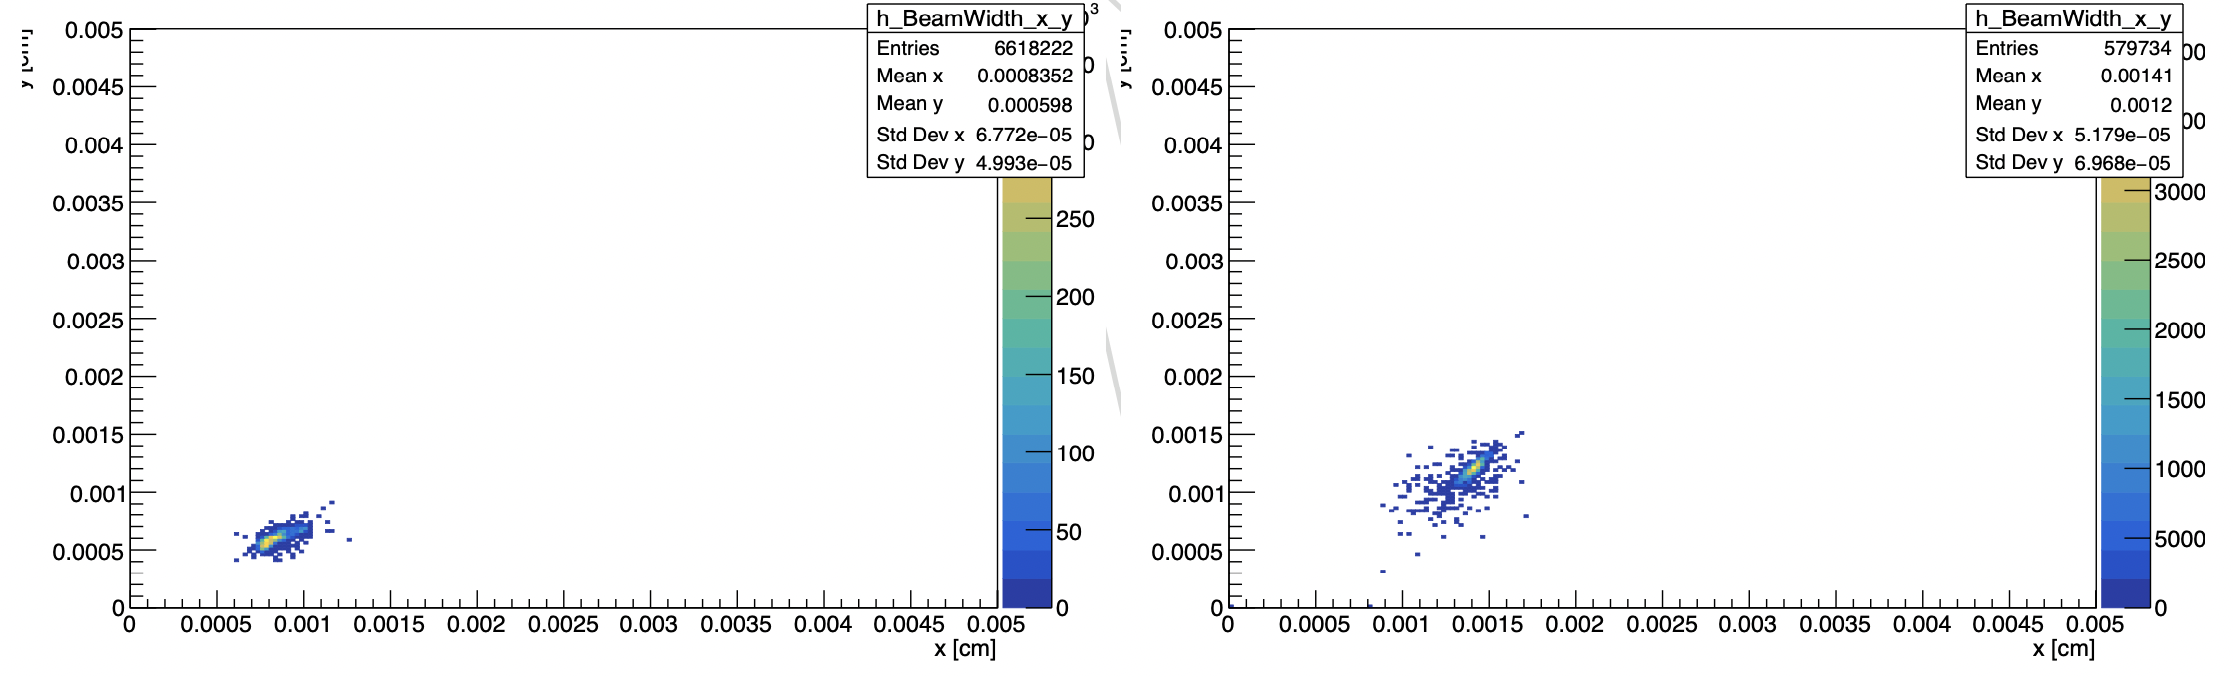
\includegraphics[width=0.96\textwidth]{figures/higgsmassmeas/vxbs/beamspot_width_2016RunG_vs_2018RunD.png}
	% \includegraphics[width=0.45\textwidth]{Figures/VXBS/2018D_VS_width_y_vs_x.pdf}
  	% \includegraphics[width=0.45\textwidth]{Figures/VXBS/2016G_VS_width_y_vs_x.pdf}
	\captionof{figure}
        [Y vs X width of beamspot for 2018 RunD \vs 2016 RunG]
        {Y vs X width of beamspot for different runs.
        \;A) 2018 Run D.
        \;B) 2016 Run G}
    \label{fig:BeamY_vs_Y}
\end{multiFigure}
Once the event is selected, the vertex+beamspot constraint is applied.

% TODO:REWORD
Muon reconstruction currently used does not take into account any information about the 
vertex production of the lepton itself. % and in the Higgs boson decay, all the leptons are prompt.
In the VX+BS approach, the four tracks from Higgs boson decay are constrained looking for a common 
vertex (VX) that must be compatible with the beamspot (BS). 
While muons information are updated after this procedure,
electrons are used only to constrain the position of the common vertex, 
leaving their kinematic information unaltered. \\
This method has been checked in DATA and in simulation, using Z boson events (60--120 GeV)
decaying into two muons: muon \pT resolution and mass resolution improves by about 5-10\%. 
This method received the green light from MuonPOG.\\ 
(Following studies within MuonPOG have been performed using UL-Summer19/20 samples.)
Figures~\ref{fig:Resolution_pT} and~\ref{fig:Resolution_eta} show muon resolution respectively 
as a function of \pT and $|\eta|$ for 2018, 2017 and 2016.
As can been seen, resolution improves by about 10$\%$ in 2018 and roughly 5$\%$ in 2016 and 2017.
\begin{multiFigure}
    \centering
        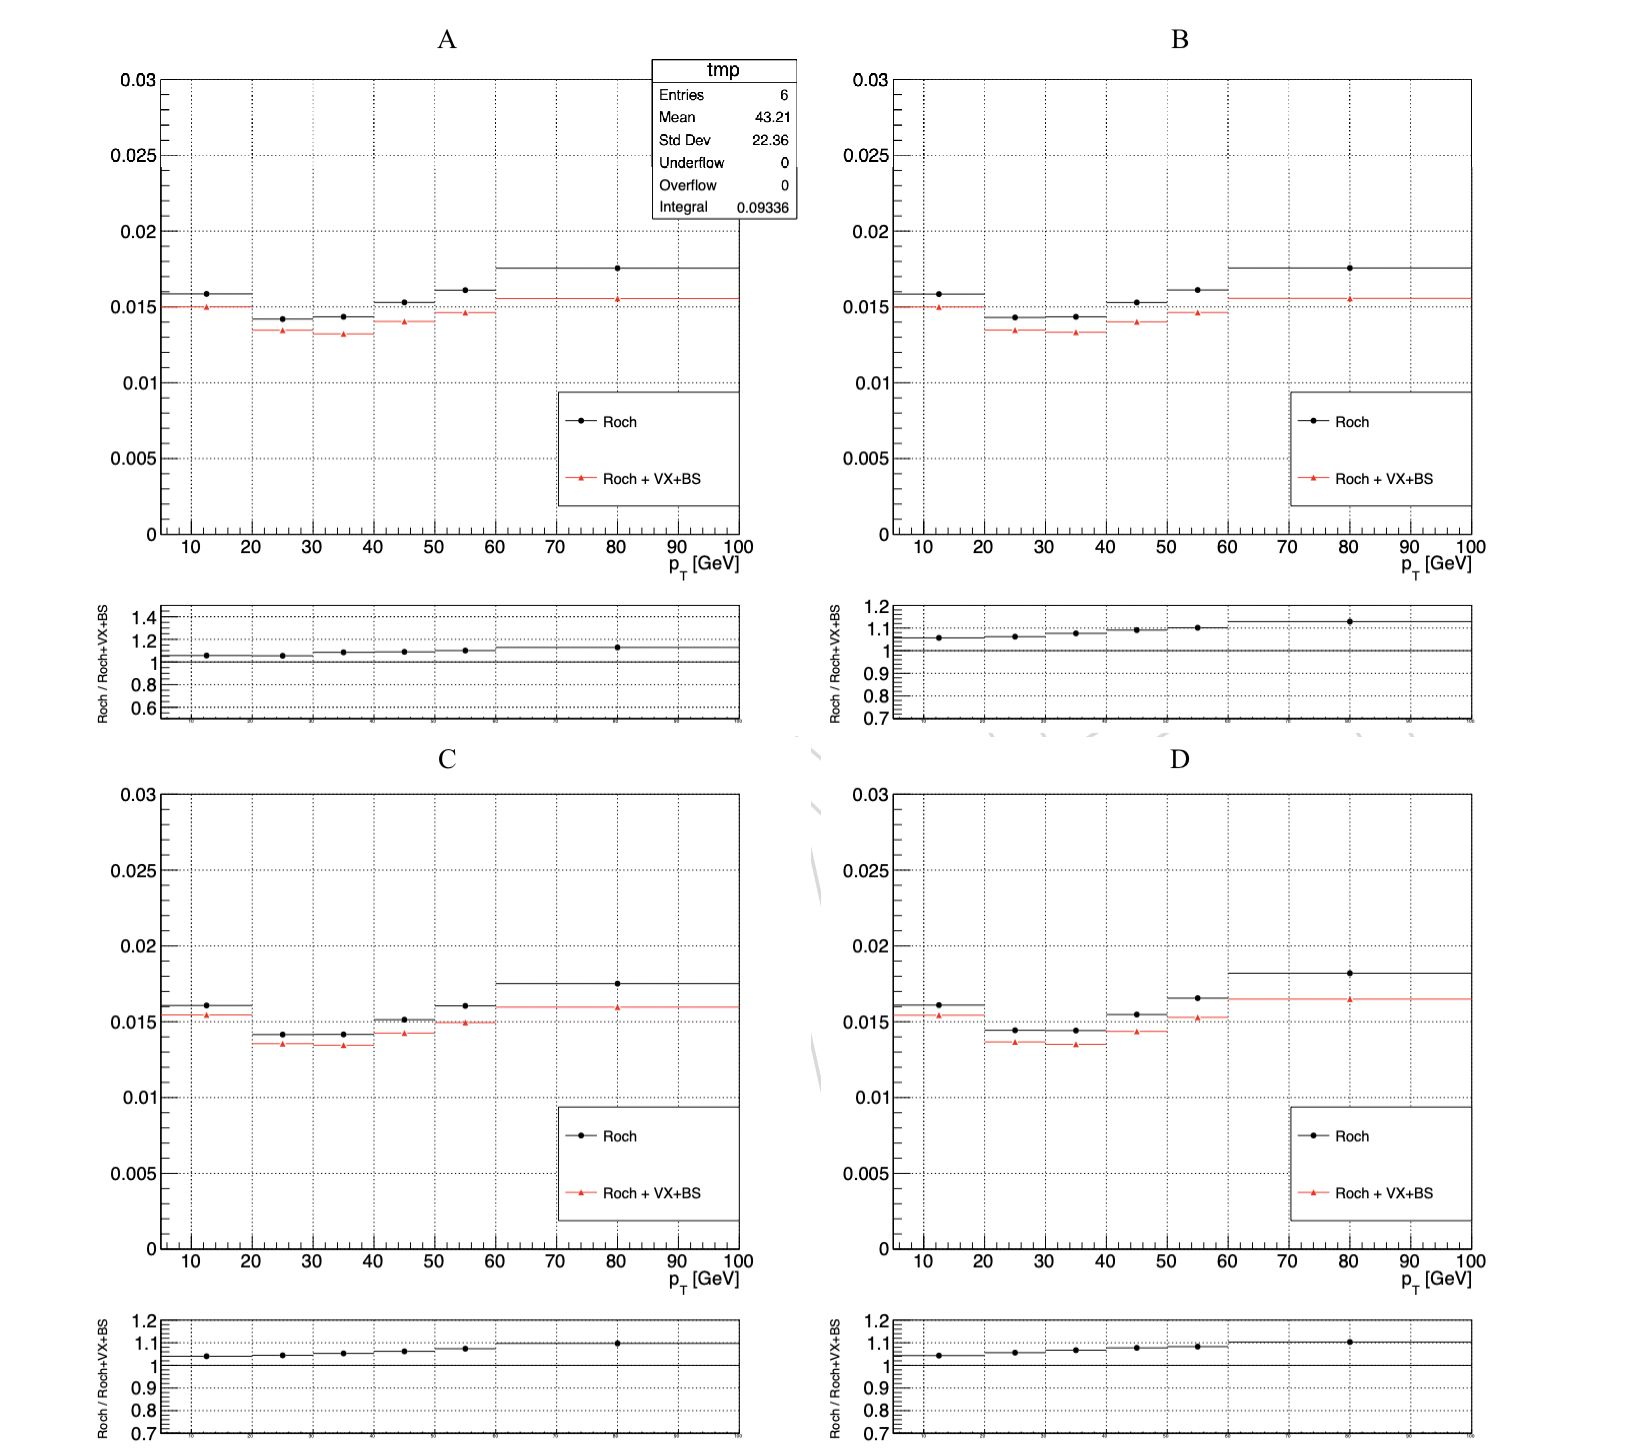
\includegraphics[width=0.96\textwidth]{figures/higgsmassmeas/vxbs/vxbs_muon_pTresol_vs_pT.png}
    \captionof{figure}
        [Muon \pT resolution as a function of \pT before and after VX+BS constraint]
        {Muon \pT resolution as a function of \pT before (black line) and after (red line) VX+BS constraint.
        \;A) 2018.
        \;B) 2017.
        \;C) 2016 post-VFP.
        \;D) 2016 pre-VFP.}
        % TODO: Use actual PDFs.
        % TODO: Split pic up properly?
\label{fig:Resolution_pT}
\end{multiFigure}
\begin{multiFigure}
    \centering
        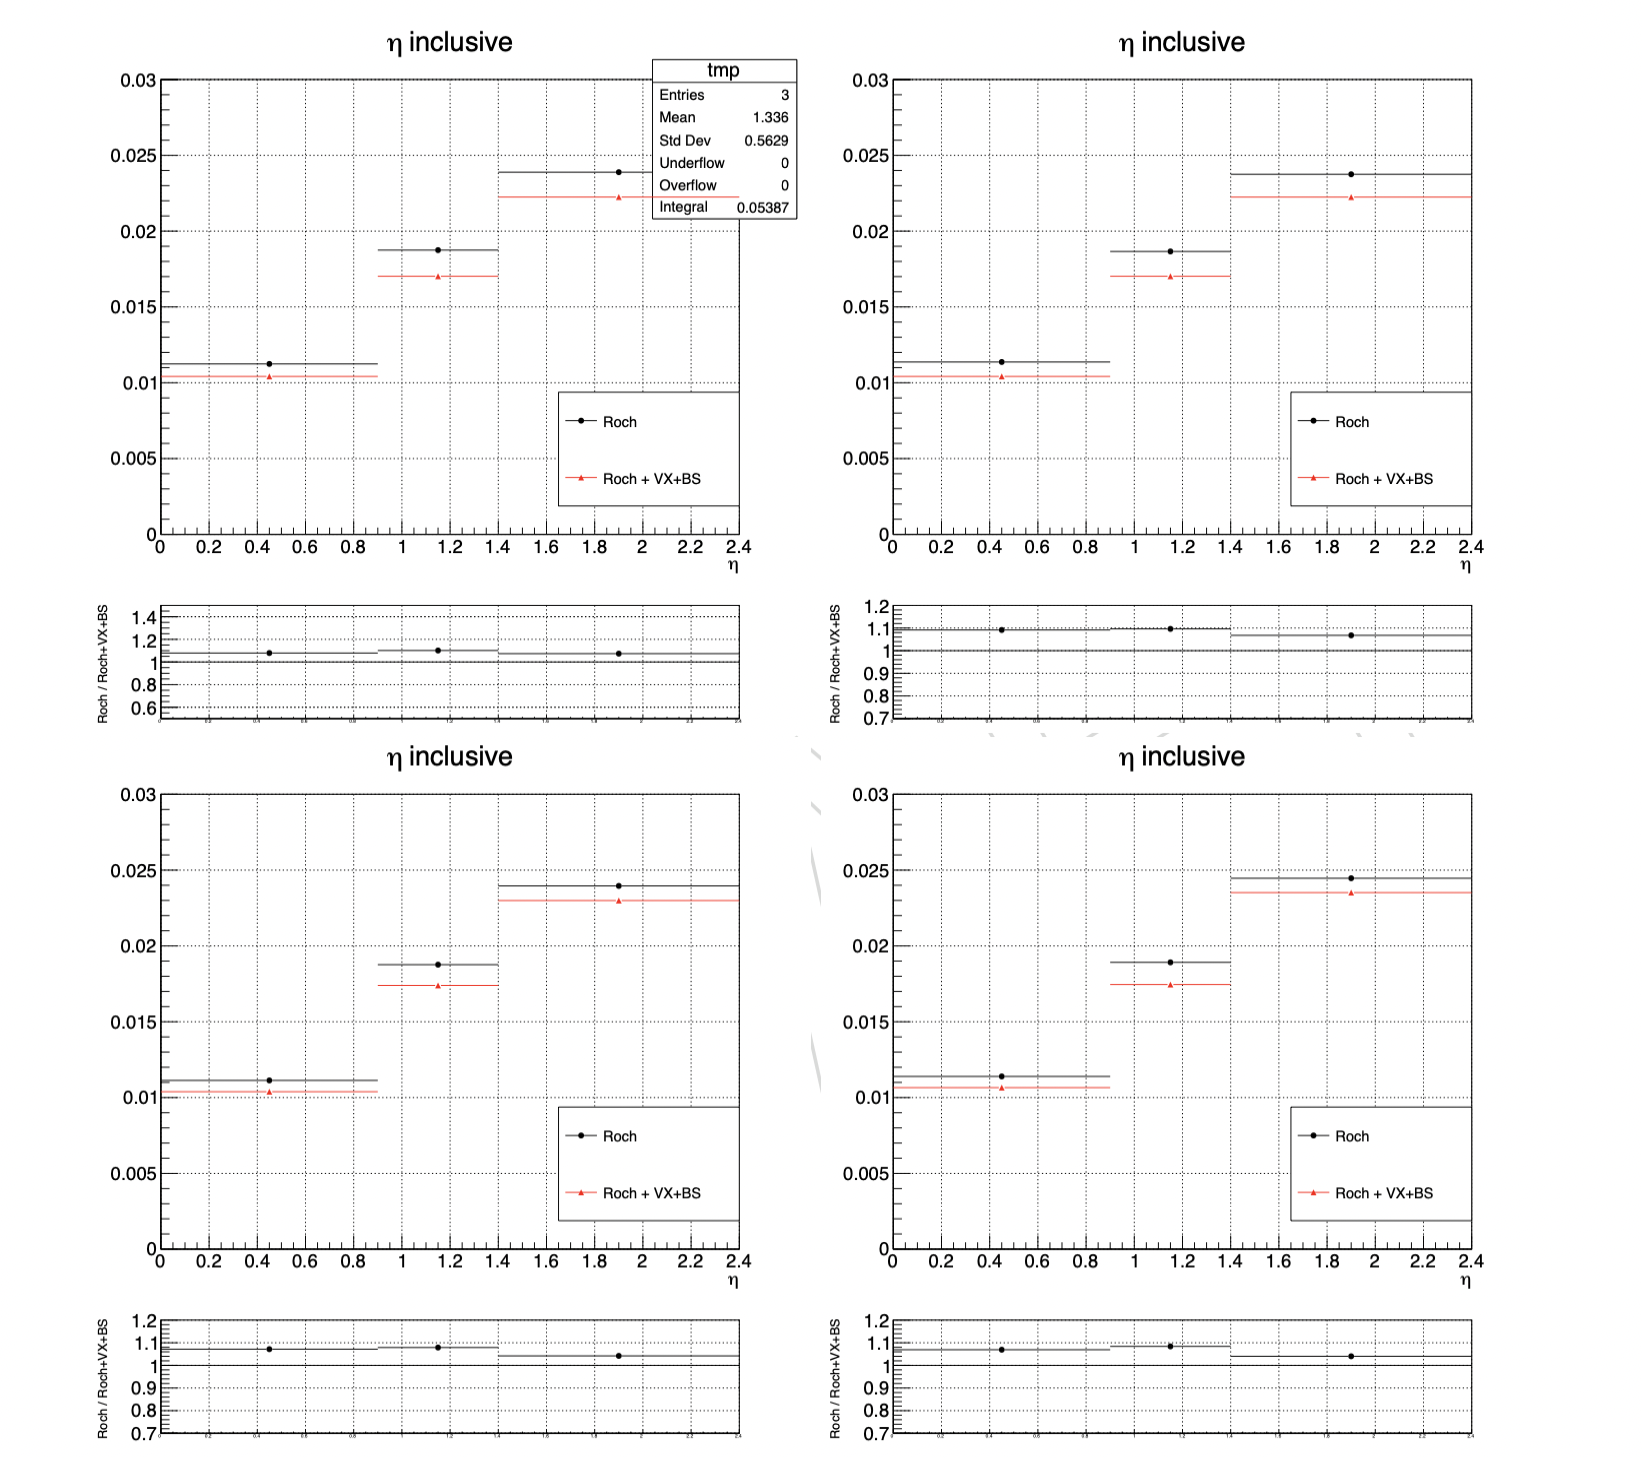
\includegraphics[width=0.96\textwidth]{figures/higgsmassmeas/vxbs/vxbs_muon_pTresol_vs_eta.png}
    \captionof{figure}
        [Muon \pT resolution as a function of \abseta before and after VX+BS constraint]
        {Muon \pT resolution as a function of \abseta before (black line) and after (red line) VX+BS constraint.
        \;A) 2018.
        \;B) 2017.
        \;C) 2016 post-VFP.
        \;D) 2016 pre-VFP.} % TODO: Use actual PDFs. Split pic up properly?
\label{fig:Resolution_eta}
\end{multiFigure}

% TODO: Find all Data-MC -> Data--MC.
Figure~\ref{UL_ZBoson_DataMC_comparison_VXBS} shows Data--MC comparison, with and without VXBS constraint.
The mean and the $\sigma$ reported on the plots are the once of the DSCB used to fit the distribution (convolved with a BW) and that simulate the detector effect.
As can been seen, the \PZ boson resolution gets improved comparably to that of the improvement of muon \pT resolution:
7\%(8\%) for 2018 DATA (MC), 5\%(4\%) for 2017, 5\%(6\%) for post-VFP and 5\%(5\%) for 2016 pre-VFP. 
\begin{multiFigure}
    \centering
        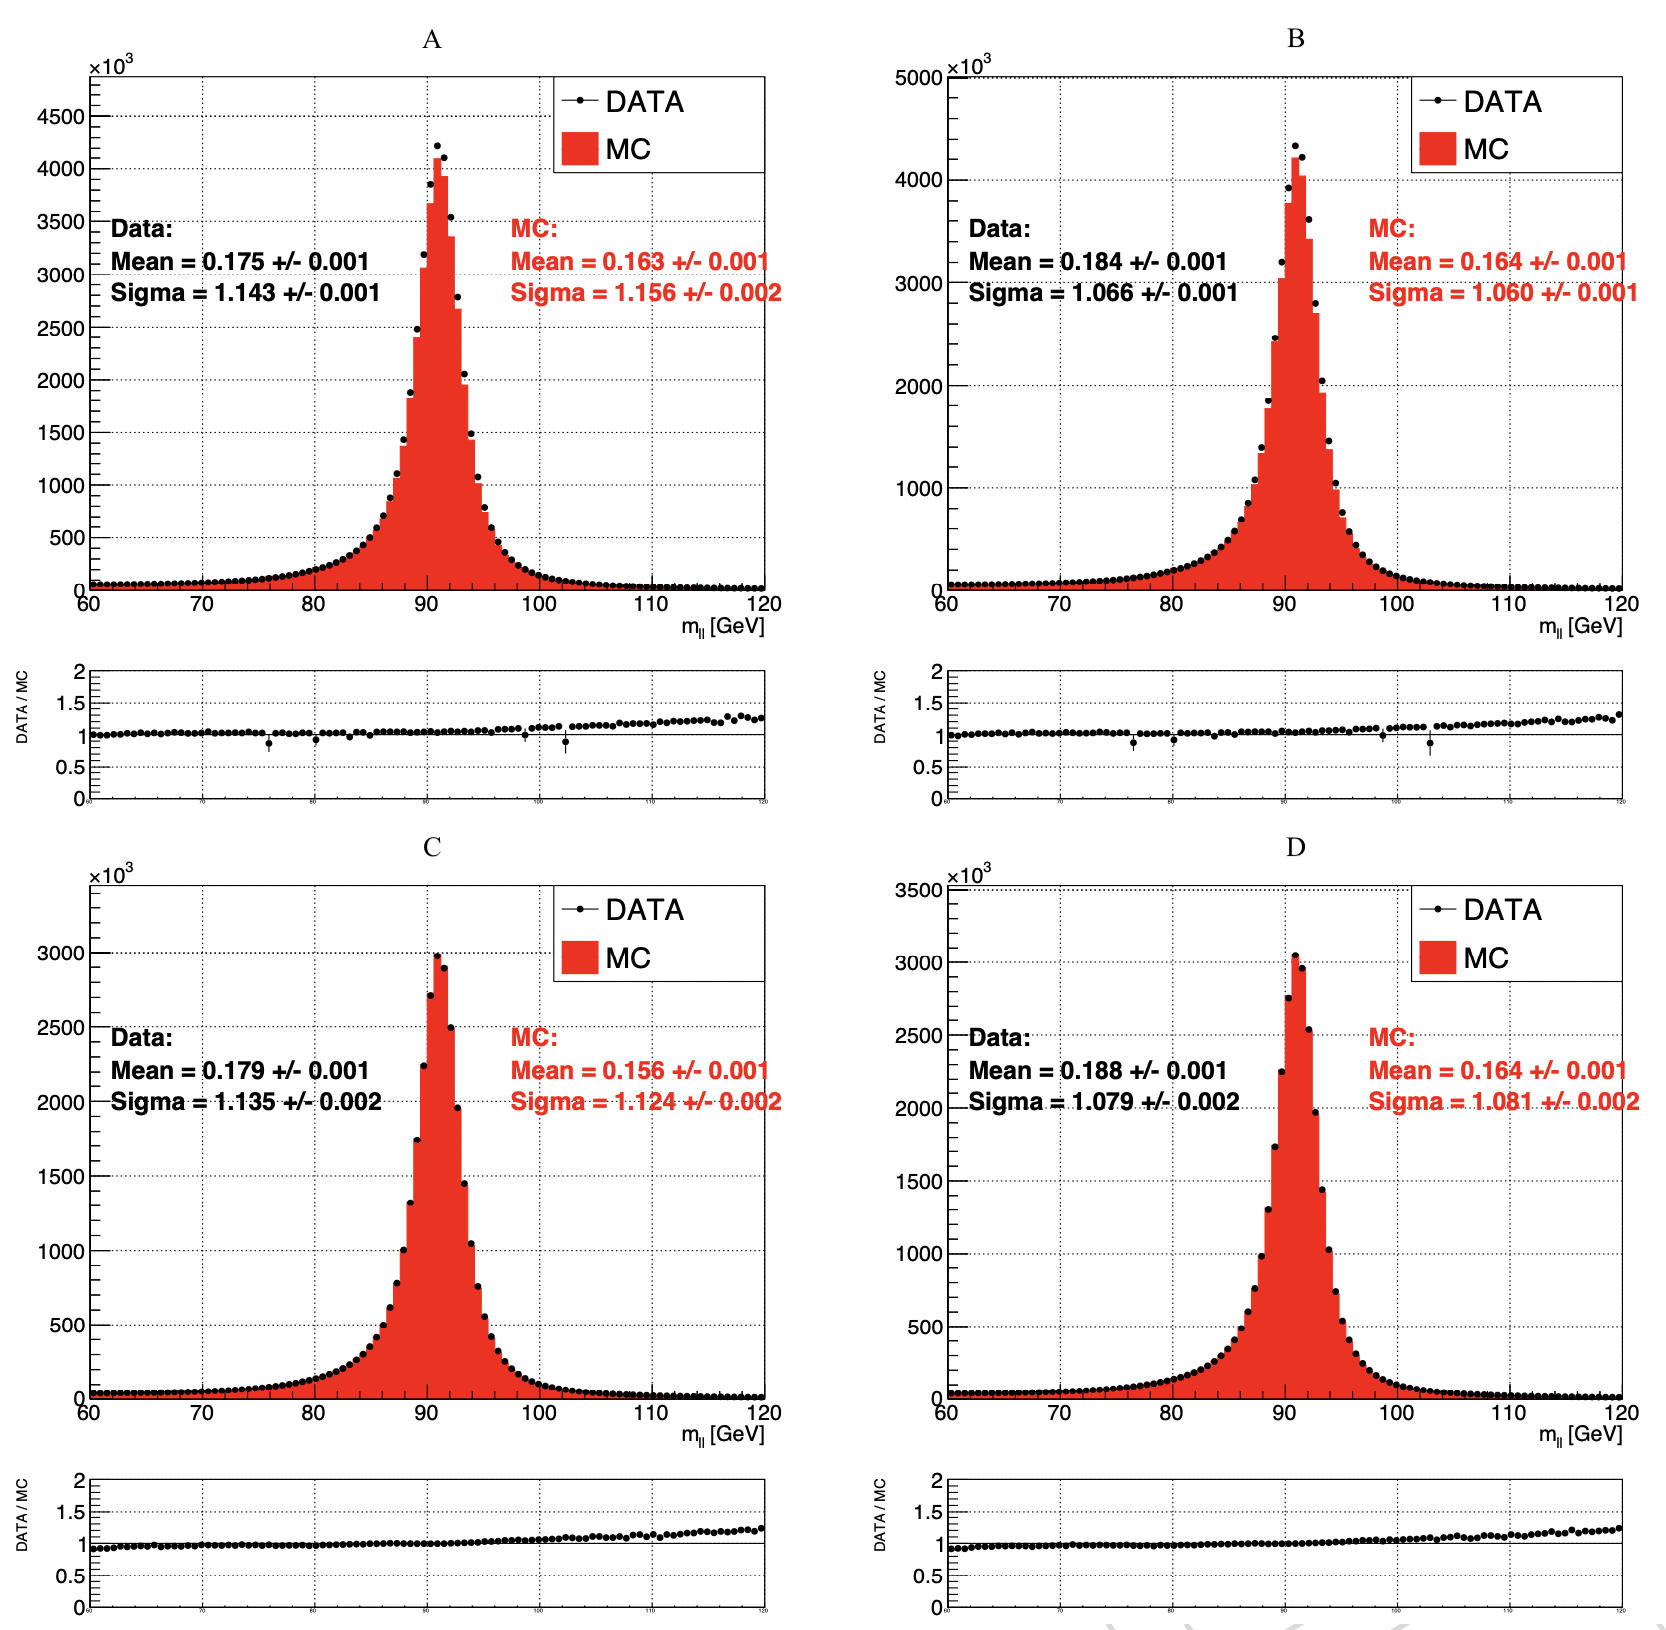
\includegraphics[width=0.96\textwidth]{figures/higgsmassmeas/vxbs/vxbs_mZdist_2017_2018.png}
	% 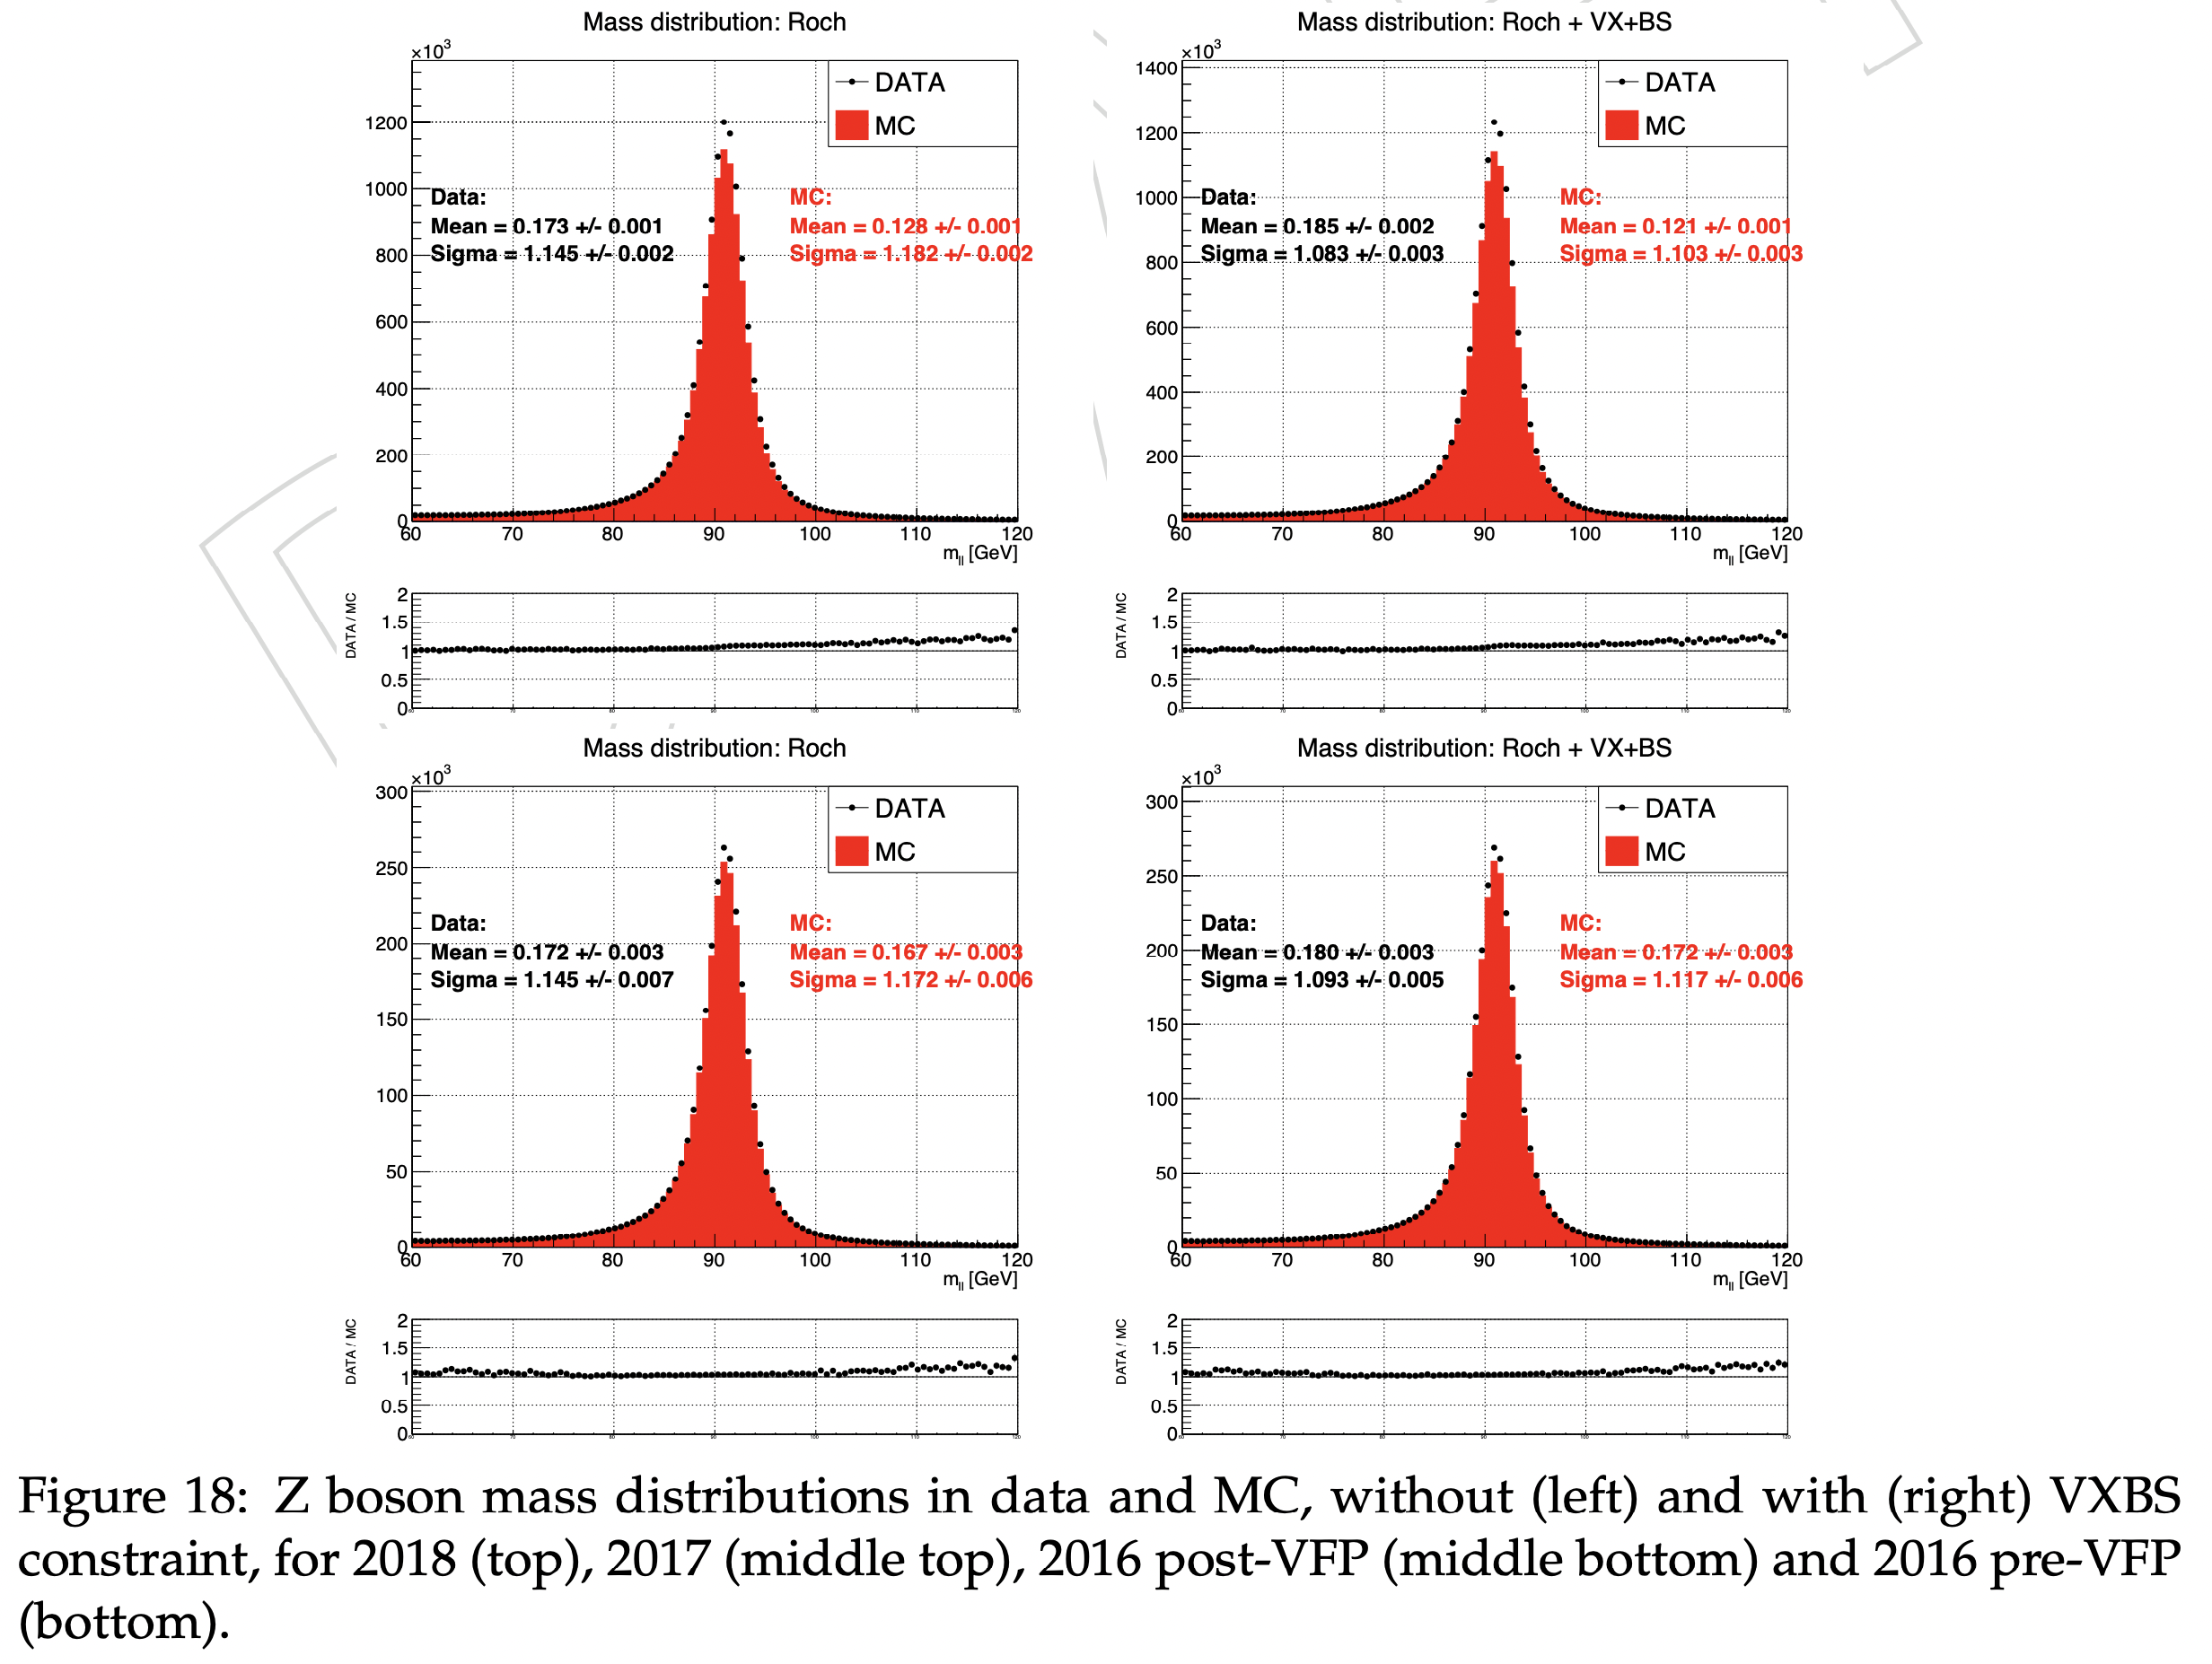
\includegraphics[width=0.96\textwidth]{figures/higgsmassmeas/vxbs/vxbs_mZdist_2016preVFP_2016postVFP.png}
    \captionof{figure}
        [\PZ boson mass distributions in data and MC, with and without VX+BS constraint]
        {\PZ boson mass distributions in data and MC, without (left) and with (right) VX+BS constraint. % TODO: REWORD 
        \;A) 2018.
        \;B) 2017.
        \;C) 2016 post-VFP.
        \;D) 2016 pre-VFP.} % TODO: Use actual PDFs. Split pic up properly?
\label{UL_ZBoson_DataMC_comparison_VXBS}
\end{multiFigure}

% More on beamspot constraint studies can be found in Appendix~\ref{app:adhoc_studies}. % TODO:Link not showing up % TODO: Fix appendix.

%=== 1D likelihood fit after VX+BS ===%
The updated invariant mass distributions, after applying the VX+BS constraint, are shown in Fig.~\ref{fig:1D_VXBS_mass_2018_ggH}.
\begin{multiFigure}
    \centering
        \addFigure{0.45}{figures/higgsmassmeas/ggH_MassDistribution/1D_VXBS_mass_2018_ggH_4mu.pdf}
        \addFigure{0.45}{figures/higgsmassmeas/ggH_MassDistribution/1D_VXBS_mass_2018_ggH_4e.pdf}
        \addFigure{0.45}{figures/higgsmassmeas/ggH_MassDistribution/1D_VXBS_mass_2018_ggH_2e2mu.pdf}
        \addFigure{0.45}{figures/higgsmassmeas/ggH_MassDistribution/1D_VXBS_mass_2018_ggH_2mu2e.pdf}
    \captionof{figure}
        [Four-lepton invariant mass distribution, after applying the VX+BS constraint]
        {Four-lepton invariant mass distribution, after applying the VX+BS constraint in the signal region ([105-140]\GeV) using ggH events, with the DSCB fit for 2018.
        \;A) 4$\mu$.    % TODO: fix symbols
        \;B) 4e.
        \;B) 2e2$\mu$.
        \;B) 2$\mu$2e.}
    \label{fig:1D_VXBS_mass_2018_ggH}
\end{multiFigure}
As can been seen, comparing these new distributions (Fig.~\ref{fig:1D_VXBS_mass_2018_ggH}, TODO) with the ones before beamspot constraint (Fig.~\ref{fig:1D_VXBS_mass_2018_ggH}, TODO), the $\sigma$ in 4$\mu$ final state has improved by 7$\%$, 4e is not affected (as expected), while mixed flavor final states show an improvement of a few percent.

\subsubsection{Expected \mH measurement uncertainties (MC)}
The expected $\mass{H}$ measurement uncertainties comparing VX+BS constraint to the baseline expectations can be seen in Table~\ref{table:1D_model_result_fs_BS} split by final state or in Table~\ref{table:1D_model_result_year_BS} split by year.

\begin{table}[ht]	
\begin{center}
    \topcaption
        [Expected Higgs boson mass uncertainty measured with 1D model, with and without VXBS, by final state]
        {Expected Higgs boson mass uncertainty measured with 1D model, with and without
        VX+BS for different final states. All mass values are given in \MeVns.
        Statistical-only results are considered at this stage of the analysis.
        }
    \begin{tabular}{ccccccc}
            \hline			
        Expected uncertainty (\MeVns)	&	4$\mu$	&	4e	&	2e2$\mu$	&2$\mu$2e	& inclusive	& Rel. Improvement \\
            \hline			
        1$D_{VXBS}$  (No bkg)	&	137	&	394	&	275	&	266	&	108 &	-4\%	\\
            1D	(No bkg) &	147	&	394	&	276	&	273	&	112	&	-	\\
        %	1$D_{VXBS}$  (No bkg)	&	144	&	466	&	313	&	291	&	116	&	-4\%	\\	
        %	1D	(No bkg) &	153	&	466	&	315	&	300	&	121 	&	- \\
            \hline
    \end{tabular}
    \label{table:1D_model_result_fs_BS}
\end{center}
\end{table}
\begin{table}[ht]	
\begin{center}
    \topcaption
        [Expected Higgs boson mass uncertainty measured with 1D model, with and without VXBS, by year]
        {Expected Higgs boson mass uncertainty measured with 1D model, with and without
        VX+BS for different years. All mass values are given in \MeVns.
        Statistical-only results are considered at this stage of the analysis.
        }
    \begin{tabular}{ccccc}
        \hline			
    Expected uncertainty (\MeVns)	&	2016 pre-VFP	&	2016 post-VFP	&	2017	&	2018	\\
        \hline			
        1$D_{VXBS}$	(No bkg)	&	291	&	301	&	198	&	162	\\
        1D (No bkg)	&	304	&	314	&	207	&	170	\\
    %	1$D_{VXBS}$	(No bkg)	&	227	&	212	&	173	\\
    %	1D (No bkg)	&	234	&	222	&	182	\\
        \hline
    \end{tabular}
    \label{table:1D_model_result_year_BS}
\end{center}
\end{table}

% \subsection{\texorpdfstring{\Zone}{Z1} Mass Constraint}  % TODO: Makes Z1 in subsection title NOT bold.
\subsection{Refitting muon and electron \pt with a \texorpdfstring{\Zone}{Z1} Mass Constraint}  % TODO: Makes Z1 in subsection title NOT bold.
% % \subsection{\texorpdfstring{\boldmath{\Zone}}{Z1} Mass Constraint} % TODO: Although \boldmath makes \subsection bold, it also makes the TOC entry bold.
\label{sec:Z1constraint}

%\subsubsection{Z1-mass line shape}
% \subsubsection{Methodology}
% TODO:REWORD, USE CONSISTENT SYMBOLS.
In order to improve the four lepton invariant mass resolution, a kinematic fit is also performed
using a mass constraint on the intermediate on-shell Z resonance, using an approach similar to the one
described previously.
% TODO:CITE
% \cite{RefToZrefit}.
The basic idea is to re-evaluate \pT of two leptons forming 
the Z bosons of the Higgs candidate, with a constraint on the reconstructed Z mass to follow 
the Z boson true lineshape. For a 125\GeV Higgs, the selected $Z_{1}$ is mostly on-shell, 
while $m_{Z_{2}}$ distribution is broad and the spread is much bigger than detector resolution. 
When considering mass measurment of 125\GeV Higgs, expected gain in resolution comes from refitting $Z_{1}$.
The likelihood to be maximized can be written as:
\[
\mathcal{L}(p_{T}^{1} , p_{T}^{2}|p_{T}^{reco1}, \sigma p_{T}^{1},p_{T}^{reco2}, \sigma p_{T}^{2}) = 
Gauss(p_{T}^{reco1}|p_{T}^{1}, \sigma p_{T}^{1}) \cdot Gauss(p_{T}^{reco2}|p_{T}^{2}, \sigma p_{T}^{2}) 
\cdot \mathcal{L}(m_{12}|\mZ,m_{H})
\]
where $p_{T}^{reco1,2}$ are the reconstructed transverse momentum of the two leptons forming the $Z_{1}$,
$\sigma_{p_{T}^{1,2}}$ are the per lepton resolution (uncertainty on \pT measurement, corrected using 
method described in \ref{sec:ebe}), $p_{T}^{1,2}$ are the observables under optimisation,
$m_{12}$ is the invariant mass calculated from $p_{T}^{1}$ and $p_{T}^{2}$. $\mathcal{L}(m_{12}|\mZ,m_{H})$
is the likelihood, given the true lineshape of $m_{Z_{1}}$. \\
%For a 125\GeV Higgs, the selected $Z_{1}$ is not always on-shell, so the Breit Wigner shape can not describe
%perfectly its lineshape at generator level. In principle, one can choose any of the $Z_{1}$ 
%lineshapes to be used in the refitting procedure. As long as all Monte Carlor samples and data
%events go through the same procedure (including the same true $Z_{1}$ lineshape), 
%no bias would be introduced.  We choose true gen level $Z_{1}$ lineshape from the SM Higgs boson sample to
%optimize the sensitivity.
For each event, the likelihood is maximized and \pT information of the refitted leptons are updated. \\
Fig.~\ref{fig:Z1_lineshape} shows the on-shell Z resonance line shape, at generator level, 
used to perform the kinematical fit, as taken from ggH 125\GeV sample. 
Events from all three years have been merged, asking for a 
$p_T > 20(10)$\GeV for (sub)leading leptons, and $|\eta|<$2.4(2.5) for $\Pmu$(e), focusing on
the reconstructed mass range of [105-140]\GeV in $m_{4l}^{RECO}$. The fit function used is a convolution
of a CB plus three different guassians.
\begin{multiFigure}
    \centering
        \addFigure{0.45}{../../higgsmassmeasurement/AN-19-248/Figures/Z1_lineshape/4mu.pdf}
        \addFigure{0.45}{../../higgsmassmeasurement/AN-19-248/Figures/Z1_lineshape/4e.pdf}
        \addFigure{0.45}{../../higgsmassmeasurement/AN-19-248/Figures/Z1_lineshape/2e2mu.pdf}
        \addFigure{0.45}{../../higgsmassmeasurement/AN-19-248/Figures/Z1_lineshape/2mu2e.pdf}
	\captionof{figure}
        [On-shell Z resonance line shape at generator level, as taken from ggH sample @ 125\GeV]
        {On-shell Z resonance line shape at generator level, as taken from ggH sample @ 125\GeV, % TODO:REWORD
        merging all three years for the 4 different final states.
        \;A) \fourmu.
        \;B) \foure.
        \;C) \twoetwomu.
        \;D) \twomutwoe.}
    \label{fig:Z1_lineshape}
\end{multiFigure}
%After this kinimatic refitting, the mass of the Z candidate, the $m_{4\ell}$, and the $\sigma_{m_{4\ell}}$
%are recalculated. The comparison of the reconstructed and refitted mass can be seen in Fig.~\ref{Z1constraint}.

% \subsection{Mass distributions}
The new invariant mass distributions, with also the constraint of the on-shell Z1 boson, are shown in 
Fig.~\ref{fig:1D_VXBS_Z1_mass_2018_ggH}.
\begin{multiFigure}
    \centering
        \addFigure{0.45}{figures/higgsmassmeas/ggH_MassDistribution/1D_VXBS_Z1_mass_2018_ggH_4mu.pdf}
        \addFigure{0.45}{figures/higgsmassmeas/ggH_MassDistribution/1D_VXBS_Z1_mass_2018_ggH_4e.pdf}
        \addFigure{0.45}{figures/higgsmassmeas/ggH_MassDistribution/1D_VXBS_Z1_mass_2018_ggH_2e2mu.pdf}
        \addFigure{0.45}{figures/higgsmassmeas/ggH_MassDistribution/1D_VXBS_Z1_mass_2018_ggH_2mu2e.pdf}
    \captionof{figure}
        [Four-lepton invariant mass distribution, with VXBS and Z1 constraint]
        {Four-lepton invariant mass distribution, with VXBS and Z1 constraint, in the signal region ([105-140]\GeV) using ggH events, with the DSCB fit for 2018: % TODO:REWORD
        \;A) \fourmu.
        \;B) \foure.
        \;C) \twoetwomu.
        \;D) \twomutwoe.} 
    \label{fig:1D_VXBS_Z1_mass_2018_ggH}
\end{multiFigure}
Comparing these new distributions (Fig.~\ref{fig:1D_VXBS_Z1_mass_2018_ggH}) with the previous ones (Fig.~\ref{fig:1D_VXBS_mass_2018_ggH}), it can be seen that the \Zone constraint has a bigger improvement in final states with on-shell Z boson decaying in to 2e (~30$\%$ improvement on $\sigma$ for \twoetwomu and 16$\%$ for \foure) while the other two final states (\fourmu and \twomutwoe) are less affected (improvement in $\sigma$ of the other of 5$\%$).

\subsubsection{Expected mH measurement uncertainties (MC) and relative improvements}
The new four-lepton mass ($m'_{4\ell}$), shown in Fig.~\ref{fig:1D_VXBS_Z1_mass_2018_ggH},
is used to rebuild the 1D likelihood function, $\mathcal{L}$($m'_{4\ell}|m_{H}$). Signal normalisation and signal parameterization are extracted following the procedure described in \ref{sec:signal_model}.
The expected \mH measurement uncertainty, is reported in \cref{table:1D_model_result_Z1} (or in \cref{table:1D_model_result_Z1_year}
splitted in years).
%===
\begin{table}[ht]	
\begin{center}
    \topcaption
        [Expected Higgs boson mass uncertainty measured with 1D model, with and without
        Z1 refit for different final states]
        {Expected Higgs boson mass uncertainty measured with 1D model, with and without
        Z1 refit for different final states. All mass values are given in \MeV.
        Statistical only results are considered at this stage of the analysis.
        }
    \begin{tabular}{ccccccc}
        \hline			
    Expected uncertainty	&	\fourmu	&	\foure	&	\twoetwomu	&\twomutwoe	& inclusive & Rel. Improvement \\
        \hline			
        1$D'_\text{VXBS}$ (No bkg)	&	129	&	357	&	223	&	255	&	99	&	-8\%	\\
        1$D_\text{VXBS}$  (No bkg)	&	137	&	394	&	275	&	266	&	108 &	-4\%	\\
    %	1$D'_\text{VXBS}$ (No bkg)	&	134	&	424	&	250	&	279	&	105	&	-9\%	\\
    %	1$D_\text{VXBS}$  (No bkg)	&	144	&	466	&	313	&	291	&	116	&	-\\	
        %\hline
    %relative improvement	&	-	&	-	&	-	&	-	&	-	\\
        \hline
\end{tabular}
\label{table:1D_model_result_Z1}
\end{center}
\end{table}
%===
\begin{table}[ht]	
\begin{center}
    \topcaption
        [Expected Higgs boson mass uncertainty measured with 1D model, with and without
        Z1 refit for different years]
        {Expected Higgs boson mass uncertainty measured with 1D model, with and without
        Z1 refit for different years. All mass values are given in \MeV.
        Statistical only results are considered at this stage of the analysis.
        }
    \begin{tabular}{ccccc}
        \hline			
    Expected uncertainty	&	2016 pre-VFP	&	2016 post-VFP	&	2017	&	2018	\\
        \hline			
        1$D'_\text{VXBS}$ (No bkg)	&	266	&	276	&	182	&	148	\\
        1$D_\text{VXBS}$	(No bkg)	&	291	&	301	&	198	&	162	\\
    %	1$D'_\text{VXBS}$ (No bkg)	&	206	&	194	&	157	\\
    %	1$D_\text{VXBS}$	(No bkg)	&	227	&	212	&	173	\\
        \hline
    \end{tabular}
    \label{table:1D_model_result_Z1_year}
\end{center}
\end{table}

% Expected mH measurement uncertainties using 3D pdf(m4l, sigma, Dkin | mH)
% with background (no systematics yet)
%\section{$D_{m_{4\ell}}$ categorization}
\subsection{Relative mass error categorization}
\label{sec:SignalParam_N_2D}
In the latest public results TODO:CITE, a 3D likelihood has been used to extract final Higgs boson mass uncertainty. 
For the full Run 2 results, a categorization based on the relative mass error is implemented.
This method will help not only in taking into account the correlation with the \Dkinbkg (see \ref{sec:DkinCorrelation}), but it will also improve the signal parameterization.
In particular, it has been found that the signal parameters of the DSCB not only depend on the mass but also on the relative mass error.\\
Starting from the raw distribution of the relative mass error, taken from ggH 125 \GeV sample, 
9 bins are defined guaranteeing an equal amount of raw events in each bin. Bin split 
is done independently for each year and for each final state. Example of the binning is given, 
for 2018, in  Fig.~\ref{Bin_splitting_2018}. First studies on categorizations can be found in TODO:CITE.
% \cite{HIG_18_002}.
\begin{figure}[!htbp]
\begin{center}
	\includegraphics[width=0.45\textwidth]{../../higgsmassmeasurement/AN-19-248/Figures/Bin_splitting/RelMassErroSplitting_4mu.pdf}
	\includegraphics[width=0.45\textwidth]{../../higgsmassmeasurement/AN-19-248/Figures/Bin_splitting/RelMassErroSplitting_4e.pdf}
  	\includegraphics[width=0.45\textwidth]{../../higgsmassmeasurement/AN-19-248/Figures/Bin_splitting/RelMassErroSplitting_2e2mu.pdf}
	\includegraphics[width=0.45\textwidth]{../../higgsmassmeasurement/AN-19-248/Figures/Bin_splitting/RelMassErroSplitting_2mu2e.pdf}
\caption{
	Relative mass error distribution for 2018 ggH sample @ 125 GeV: black lines show 
	the bins used for the categorization.}
\label{Bin_splitting_2018}
\end{center}
\end{figure}
To extract mass measurement using categorization, the signal is modelled independently in each bin, 
obtaining final measurements combining data cards. \\
Examples of the signal parameterization for 2018 are shown in 
Fig.~\ref{signal_lineshape_2018_4mu}(4$\mu$),
 \ref{signal_lineshape_2018_4e} (4e), 
 \ref{signal_lineshape_2018_2e2mu} (2e2$\mu$) and \ref{signal_lineshape_2018_2mu2e} (2$\mu$2e). 
 Each figure shows the fit of the 125 \GeV ggH sample (in blue, top left) and
the simultaneous fits of the all five mass points (red scale) in few random bins.
%Fig.~\ref{signal_lineshape_2016}(2$\mu$2e 2016),
% \ref{signal_lineshape_2017} (2e2$\mu$ 2017), 
% \ref{signal_lineshape_2018_1} (4e 2018) and  \ref{signal_lineshape_2018_2} (4$\mu$ 2018). 
%for 125 GeV sample, and in  Fig.~\ref{signal_lineshape_2016_full_1}, 
%\ref{signal_lineshape_2016_full_2}, \ref{signal_lineshape_2017_full_1}, 
%\ref{signal_lineshape_2017_full_2}, \ref{signal_lineshape_2018_full_1} and  
%\ref{signal_lineshape_2018_full_2}, for the simultaneous fits.
\begin{figure}[!htbp]
\begin{center}
	\includegraphics[width=0.45\textwidth]{../../higgsmassmeasurement/AN-19-248/Figures/Categorisation/DSCB_4mu_ggF_2018_2.pdf}
	\includegraphics[width=0.45\textwidth]{../../higgsmassmeasurement/AN-19-248/Figures/Categorisation/DSCB_4mu_ggF_2018_3.pdf}
	\includegraphics[width=0.45\textwidth]{../../higgsmassmeasurement/AN-19-248/Figures/Categorisation/DSCB_4mu_ggF_2018_8.pdf}
	\includegraphics[width=0.45\textwidth]{../../higgsmassmeasurement/AN-19-248/Figures/Categorisation/DSCB_4mu_ggF_2018_9.pdf}
\caption{
Fit examples for four $D'^{VXBS}_{m_{4\ell}}$ bins (2nd, 3rd, 8th, and 9th) 
for 4$\mu$ 2018. Top left: 125 GeV sample only fit. The others plots stand for the simultaneous 
fit of all the mass points: starting from top right respectively 125, 120, 124, 126, 130 GeV.}
\label{signal_lineshape_2018_4mu}
\end{center}
\end{figure}

\begin{figure}[!htbp]
\begin{center}
	\includegraphics[width=0.45\textwidth]{../../higgsmassmeasurement/AN-19-248/Figures/Categorisation/DSCB_4e_ggF_2018_1.pdf}
	\includegraphics[width=0.45\textwidth]{../../higgsmassmeasurement/AN-19-248/Figures/Categorisation/DSCB_4e_ggF_2018_2.pdf}
	\includegraphics[width=0.45\textwidth]{../../higgsmassmeasurement/AN-19-248/Figures/Categorisation/DSCB_4e_ggF_2018_5.pdf}
	\includegraphics[width=0.45\textwidth]{../../higgsmassmeasurement/AN-19-248/Figures/Categorisation/DSCB_4e_ggF_2018_9.pdf}
\caption{
Fit examples for four $D'^{VXBS}_{m_{4\ell}}$ bins (1st, 2nd, 5th, and 9th) 
for 4e 2018. Top left: 125 GeV sample only fit. The others plots stand for the simultaneous 
fit of all the mass points: starting from top right respectively 125, 120, 124, 126, 130 GeV.}
\label{signal_lineshape_2018_4e}
\end{center}
\end{figure}

\begin{figure}[!htbp]
\begin{center}
	\includegraphics[width=0.45\textwidth]{../../higgsmassmeasurement/AN-19-248/Figures/Categorisation/DSCB_2e2mu_ggF_2018_1.pdf}
	\includegraphics[width=0.45\textwidth]{../../higgsmassmeasurement/AN-19-248/Figures/Categorisation/DSCB_2e2mu_ggF_2018_3.pdf}
	\includegraphics[width=0.45\textwidth]{../../higgsmassmeasurement/AN-19-248/Figures/Categorisation/DSCB_2e2mu_ggF_2018_7.pdf}
	\includegraphics[width=0.45\textwidth]{../../higgsmassmeasurement/AN-19-248/Figures/Categorisation/DSCB_2e2mu_ggF_2018_9.pdf}
\caption{
Fit examples for four $D'^{VXBS}_{m_{4\ell}}$ bins (1st, 3rd, 7th, and 9th) 
for 2e2$\mu$ 2018. Top left: 125 GeV sample only fit. The others plots stand for the simultaneous 
fit of all the mass points: starting from top right respectively 125, 120, 124, 126, 130 GeV.}
\label{signal_lineshape_2018_2e2mu}
\end{center}
\end{figure}

\begin{figure}[!htbp]
\begin{center}
	\includegraphics[width=0.45\textwidth]{../../higgsmassmeasurement/AN-19-248/Figures/Categorisation/DSCB_2mu2e_ggF_2018_1.pdf}
	\includegraphics[width=0.45\textwidth]{../../higgsmassmeasurement/AN-19-248/Figures/Categorisation/DSCB_2mu2e_ggF_2018_4.pdf}
	\includegraphics[width=0.45\textwidth]{../../higgsmassmeasurement/AN-19-248/Figures/Categorisation/DSCB_2mu2e_ggF_2018_6.pdf}
	\includegraphics[width=0.45\textwidth]{../../higgsmassmeasurement/AN-19-248/Figures/Categorisation/DSCB_2mu2e_ggF_2018_9.pdf}
\caption{
Fit examples for four $D'^{VXBS}_{m_{4\ell}}$ bins (1st, 4th, 6th, and 9th) 
for 2$\mu$2e 2018. Top left: 125 GeV sample only fit. The others plots stand for the simultaneous 
fit of all the mass points: starting from top right respectively 125, 120, 124, 126, 130 GeV.}
\label{signal_lineshape_2018_2mu2e}
\end{center}
\end{figure}
Looking in each bin at the parameter mean of the DSCB function, used to fit the 125 \GeV sample, 
(Fig.~\ref{MeanDependence}), it can be seen that if in 4$\mu$ final state (black dots) the mean
is quite stable, in the 4e (in red) and 2e2$\mu$ (green) final states, it shifts towards lower values
($\mathcal{O}$({GeV})). Categorization will help in properly describe the Higgs boson line shape
not only as a function of mass but also as a function of mass resolution.
% \footnote{As we went 
% through this exercise, we also uncovered a minor bug in how $f(m_{4\ell}, \sigma_{m_{4\ell}} | m_H)$ 
% was built in the past; the bug affected $4e$ and, 
% to a lesser degree, $2e2\mu$ final states.}

%This could be seen in Fig.~\ref{Mass_1D_vs_1Derr} where a direct comparison of the 
%1D mass distribution is compared with the as distribution obtained after the convolution with the 
%relative mass error. Looking in particular at 4e and 2e2$\mu$ final state, the two distributions
%show differences; on the opposite, in the case of 4$\mu$ and 24$\mu$2e final states, 
%the two distributions are quite similar. 
\begin{figure}[!htbp]
\begin{center}
		\includegraphics[width=0.45\textwidth]{../../higgsmassmeasurement/AN-19-248/Figures/Categorisation/MeanDependenceFromSigma_20160.pdf}
		\includegraphics[width=0.45\textwidth]{../../higgsmassmeasurement/AN-19-248/Figures/Categorisation/MeanDependenceFromSigma_20165.pdf}
		\includegraphics[width=0.45\textwidth]{../../higgsmassmeasurement/AN-19-248/Figures/Categorisation/MeanDependenceFromSigma_2017.pdf}
		\includegraphics[width=0.45\textwidth]{../../higgsmassmeasurement/AN-19-248/Figures/Categorisation/MeanDependenceFromSigma_2018.pdf}
\caption{
DSCB mean values as a function of mass resolution for the four different final states: 4$\mu$ (black),
4e (red), 2e2$\mu$ (green) and 2$\mu$2e (blue). Each bin on the x axis stands for a bin 
in categorization (moving from left to right, the relative mass error comes bigger). 
Top 2016 (left pre-VFP, right post-VFP), bottom left 2017, bottom right 2018.}
\label{MeanDependence}
\end{center}
\end{figure}
Finally, examples of the fits for normalisation can be observed in 
Fig.~\ref{signal_normalization_20160} (2016 pre-VFP ggH),
Fig.~\ref{signal_normalization_20165} (2016 post-VFP ggH), 
\ref{signal_normalization_2017} (2017 ggH) and 
\ref{signal_normalization_2018} (2018 ggH)
\begin{figure}[!htbp]
\begin{center}
		\includegraphics[width=0.45\textwidth]{../../higgsmassmeasurement/AN-19-248/Figures/Categorisation/Yield_ggF_20160.pdf}
\caption{
Normalization fit for ggH 2016 pre-VFP, for different decay channels, as a function
of mass, for the 9 bins of $D'^{VXBS}_{m_{4\ell}}$.}
\label{signal_normalization_20160}
\end{center}
\end{figure}
\begin{figure}[!htbp]
\begin{center}
		\includegraphics[width=0.45\textwidth]{../../higgsmassmeasurement/AN-19-248/Figures/Categorisation/Yield_ggF_20165.pdf}
\caption{
Normalization fit for ggH 2016 post-VFP, for different decay channels, as a function
of mass, for the 9 bins of $D'^{VXBS}_{m_{4\ell}}$.}
\label{signal_normalization_20165}
\end{center}
\end{figure}
\begin{figure}[!htbp]
\begin{center}
		\includegraphics[width=0.45\textwidth]{../../higgsmassmeasurement/AN-19-248/Figures/Categorisation/Yield_ggF_2017.pdf}
\caption{
Normalization fit for ggH 2017, for different decay channels, as a function
of mass, for the 9 bins of $D'^{VXBS}_{m_{4\ell}}$.}
\label{signal_normalization_2017}
\end{center}
\end{figure}
\begin{figure}[!htbp]
\begin{center}
		\includegraphics[width=0.5\textwidth]{../../higgsmassmeasurement/AN-19-248/Figures/Categorisation/Yield_ggF_2018.pdf}
\caption{
Normalization fit for ggH 2018, for different decay channels, as a function
of mass, for the 9 bins of $D'^{VXBS}_{m_{4\ell}}$.}
\label{signal_normalization_2018}
\end{center}
\end{figure}

%In Fig.~\ref{Mass_1D_vs_1Derr_categorization} it can be seen the comparison of 1D and 1Derr
%mass distribution for different final state but now in several \textbf{mass error} bins: now, the
%agreement is quite good in all final states.
%\begin{figure}[!htbp]
%\begin{center}
%		\includegraphics[width=0.35\textwidth]{../../higgsmassmeasurement/AN-19-248/Figures/Placeholder.png}
%\caption{
%Comparison of the mass distribution from 1D (green) and 1Derr (black)
%models in different \textbf{mass error} bins for .... 
%}
%\label{Mass_1D_vs_1Derr_categorization}
%\end{center}
%\end{figure}

\subsubsection{Result using categorization in 1D model}
%The mass error uncertainty evaluated in \ref{sec:EBE} is combined with the four-lepton mass to built
%a two-dimentional likelihood function, $\mathcal{L}$($m_{4\ell}$, \massUnc$|m_{H}$), where again 
%$m_{H}$ is fixed to the value of 125 GeV. \\
%\tablename~\ref{table:2D_model_result_year} shows inclusive results compared with 1D result
%for each year.
The expected $\mass{H}$ measurement uncertainty, in case of no-bkg and no-syst,
implementing the categorization, is reported in \tablename~\ref{table:2D_model_result}
split for different final state and in \tablename~\ref{table:2D_model_result_year} for different
years.
\begin{table}[ht]	
\begin{center}
    \topcaption{Expected Higgs boson mass uncertainty measured implementing the categorization,
    for different final state.
    All mass values are given in \MeV.  
    Statistical only results are considered at this stage of the analysis.
    }
    \begin{tabular}{ccccccc}
    \hline			
    Expected uncertainty	&	4$\mu$	&	4e	&	2e2$\mu$	&2$\mu$2e	& inclusive & Rel. Improvement \\
    \hline			
        N-1$D'_{VXBS}$ (No bkg)	&	124	&	319	&	203	&	236	&	92	&	-6\%	\\
        1$D'_{VXBS}$ (No bkg)	&	129	&	357	&	223	&	255	&	99	&	-8\%	\\
    %	N-1$D'_{VXBS}$ (No bkg)	&	128	&	371	&	227	&	253	&	98	&	-7\%	\\
    %	1$D'_{VXBS}$ (No bkg)	&	134	&	424	&	250	&	279	&	105	&	-	\\
    \hline
    %relative improvement	&	-	&	-	&	-	&	-	&	-	\\
    %\hline
    \end{tabular}
\label{table:2D_model_result}
\end{center}
\end{table}
\begin{table}[ht]	
\begin{center}
    \caption{Expected Higgs boson mass uncertainty measured implementing the categorization,
    for different years.
    All mass values are given in \MeV.  
    Statistical only results are considered at this stage of the analysis.
    }
    \begin{tabular}{ccccc} % TODO: Add total uncertainty in final column on right-hand side?
    \hline			
    Expected uncertainty	&	2016 pre-VFP	&	2016 post-VFP	&	2017	&	2018	\\
    \hline			
        N-1$D'_{VXBS}$ (no-bkg)	&	247	&	255	&	170	&	140	\\
        1$D'_{VXBS}$ (No bkg)	&	266	&	276	&	182	&	148	\\
    %	N-1$D'_{VXBS}$ (no-bkg)	&	192	&	180	&	147	\\
    %	1$D'_{VXBS}$ (No bkg)	&	206	&	194	&	157	\\
    \hline
    \end{tabular}
    \label{table:2D_model_result_year}
\end{center}
\end{table}

